\cleardoublepage

\chapter{Eigenvectors and eigenvalues}
\pagestyle{fancy}
\label{chapter:eigenvectors}

In the first chapter, we took what I think is the most intuitive route to defining PCA: framing the method in terms of \emph{reconstruction error}. The solution method we used wasn't very efficient or stable, and some parts of the ``why'' question were left unresolved, but we answered the ``how'' question well enough to show the method in action and hopefully convince you that it's worth digging a little deeper.

We'll start by tying up one of the loose ends from the last chapter. There, we defined PCA in terms of reconstruction error, but most other explanations instead  define it in terms of \textbf{variance maximization}. 

I started with the reconstruction error, since it requires fewer assumptions, and the required assumptions feel more intuitive. However, to explain the details of what happens under the hood, the variance perspective is more helpful, so we'll start by adding that to our toolbelt.

\section[Min. reconstruction is max. variance]{Minimal reconstruction error is maximal variance}

In the previous chapter, we defined PCA as a solution to the following problem: for a mean-centered set of instances \(\mbx_\gc{i}\) find a sequence of \(\rc{k}\)  unit vectors \(\rc{\mbw_1}, \ldots, \rc{\mbw_k}\) where each unit vector is defined by

\[
\;\;\;\;\;\;\;\; \rc{\mbw_r} = 
\begin{cases} 
	&\argmax{\rc{\mbw}} \sum_\gc{i} \|\mbx_\gc{i}^T\rc{\mbw}\rc{\mbw} - \mbx_\gc{i}\|^2 \\
	&\;\;\;\;\;\;\text{such that } \rc{\mbw}^T\rc{\mbw} = 1 \hfill \hspace{2em}\bc{\text{(a)}}\\
	&\;\;\;\;\;\;\text{and } \rc{\mbw}^T\rc{\mbw_j} = 0 \text{ for } \rc{j} \in [1 \ldots \rc{r}-1] \hfill \hspace{2em}\bc{\text{(b)}}
\end{cases}
\]

That is, each unit vector defines an approximation of \(\mbx_\gc{i}\), and the objective is to keep the distance between the reconstruction and the original instance as small as possible, while ensuring that \bc{(a)} the vector is a unit vector, and \bc{(b)} the vector is orthogonal to all preceding vectors.

The variance maximization objective takes the same form, but instead of minimizing the reconstruction error, it chooses \(\rc{\mbw}\) to \emph{maximize} the variance of the data projected onto \(\rc{\mbw}\). 

As in the previous chapter, we'll start with the one-dimensional case. We will choose a single unit vector \(\rc{\mbw}\) and project the data onto it orthogonally. That means that for every instance \(\mbx_\gc{i}\), we get a single number \(z_\gc{i}\) which is defined by \(\mbx_\gc{i}^T\rc{\mbw}\).
 
This time, our objective is to choose \(\rc{\mbw}\) so that the variance among the set of \(z_\gc{i}\) is maximized. That means that in this image
\vspace{-0.1em}
\begin{figure}[H]
	\centerline{
	\includesvg[width=0.8\textwidth]{./images/pca/random-w.svg}
	}
\end{figure}
\vspace{-1em}
%<figure class="narrow">
%<img src="/images/pca/random-w.svg" />
%</figure>
\noindent we want to choose \(\rc{\mbw}\) so that the red points are spread out as widely as possible.

Why is this the same as choosing the \(\rc{\mbw}\) that minimizes the reconstruction error? It's easy to see this if we draw a a diagram for a single instance.

\begin{figure}[H]
	\centerline{
	\includesvg[width=1\textwidth]{./images/pca/recvar-diagram.svg}
	}
\end{figure}

%<figure class="narrow">
%<img src="/images/pca/recvar-diagram.svg" />
%</figure>

Note that \(\rc{\mbw}\) is a unit vector, so for the length of the bottom edge of the triangle we have  \(\|\mbx'_\gc{i}\| = \|\rc{\mbw}z_\gc{i}\| = z_\gc{i}\).


By the Pythagoras, \(\|\mbx_\gc{i}\|^2 = \|\bc{\mbr}\|^2 + {z_\gc{i}}^2\). The vector \(\mbx_\gc{i}\) remains constant, since that is given by the data. The only thing we change is the direction of the vector \(\rc{\mbw}\). If we change that to decrease the reconstruction error \(\|\bc{\mbr}\|\), the distance \(z_\gc{i}\) must decrease. The sum of the squares of all \(\mbz_\gc{i}\)'s is the variance of the data.

%\begin{aside}
%I first learned about the equivalence between variance maximization and reconstruction error minimization from  by <a href="http://alexhwilliams.info/">Alex Williams</a>, which uses a similar diagram.
%\end{aside}

Thus, the first principal component is the vector \(\rc{\mbw}\) for which the data has maximum variance when projected onto \(\rc{\mbw}\). For the sake of completeness, let's work this into a proper proof. There's some technical stuff coming up, so we had better get into a more formal mindset.

\begin{theorem}[Equivalence of error and variance optimization.]
The vector \(\rc{\mbw}\) that minimizes the reconstruction error among the reconstructed instances \(\mbx'_\gc{i}\), maximizes the variance among the projections \(z_\gc{i}\).
\end{theorem}
\begin{proof}
The maximal variance objective can be stated as

\begin{align*}
&\argmax{\rc{\mbw}}\; \kc{\frac{1}{n}} \sum_\gc{i} (\bar z - z_\gc{i})^2 \p
\end{align*}

The objective inside the argmax is simply the definition of variance. We can drop the constant multiplier \(\kc{1/n}\), since it doesn't affect where the maximum is. We can show that \(\bar z\), the mean of the projections is 0:
\[
\bar z = \kc{\frac{1}{n}}\sum_\gc{i} \rc{\mbw}^T\mbx_\gc{i} = \rc{\mbw}^T\left( \kc{\frac{1}{n}} \sum_\gc{i} \mbx_\gc{i}\right) = \rc{\mbw}^T \mathbf{0} \p
\]

\begin{aside}The last step follows from the assumption that the data is mean-centered.\end{aside}


Thus our objective simplifies to

\begin{align*}
&\argmax{\rc{\mbw}} \sum_\gc{i} {\mbz_\gc{i}}^2 \p
\end{align*}

From our diagram above, we know that \(\|\mbx_\gc{i}\|^2 = \|\bc{\mbr}\|^2 + z_\gc{i}^2\), or, equivalently

\begin{align*}
\|\mbx_\gc{i}\|^2 &= \|\bc{\mbx_\gc{i} - \mbx'_\gc{i}}\|^2 + z_\gc{i}^2 \\
z_\gc{i}^2 &= \|\mbx_\gc{i}\|^2 - \|\bc{\mbx_\gc{i} - \mbx'_{\gc{i}}}\|^2 \p
\end{align*}

Filling this in to the optimization objective, we get

\begin{align*}
&\argmax{\rc{\mbw}} \sum_\gc{i} \kc{||\mbx_i||^2} \oc{-} ||\mbx_\gc{i} - \mbx_\gc{i}'||^2 \p
\end{align*}

where \(\kc{\|\mbx_i\|^2}\) is a constant we can remove without affecting the maximum and removing \oc{the minus} turns the maximum into a minimum. Thus, we end up with 

\begin{align*}
&\argmin{\rc{\mbw}} \sum_\gc{i} ||\mbx_\gc{i} - \mbx'_\gc{i}||^2
\end{align*}

which is the objective for minimizing the reconstruction loss. \hfill\qed

\end{proof}

The rest of the procedure is the same as before. Once we've chosen \(\rc{\mbw_1}\) to maximize the variance, we choose \(\rc{\mbw_2}\) to maximize the variance and to be orthogonal to \(\rc{\mbw_1}\), we choose \(\rc{\mbw_3}\) to maximize the variance and to be orthogonal to  \(\rc{\mbw_1}\) and to  \(\rc{\mbw_2}\) and so on.

In the previous chapter, we also defined a \textbf{combined problem}, which combined all the vectors together in one optimization objective. We can work out an equivalent for the variance perspective (the proof is in Section~\ref{section:ch2-app} of the appendix). 

\begin{theorem}[Equivalence of combined optimization.] The combined problem for reconstruction error minimization.
\begin{align*}
&\argmin{\rc{\mbW}} \sum_\gc{i} \|\mbx_\gc{i} - \mbx'_\gc{i}\|\\
&\;\;\;\text{such that } \rc{\mbW}^T\rc{\mbW} = \mbI\\
\end{align*}
is equivalent to the following variance maximization problem
\begin{align*}
&\argmax{\rc{\mbW}} \sum_{\gc{i}, \rc{r}} {z_{\gc{i}\rc{r}}}^2 \;\;\;\;\;\text{with } z_{\gc{i}\rc{r}} = \rc{\mbw_r}^T\mbx_\gc{i}\\
&\;\;\;\text{such that } \rc{\mbW}^T\rc{\mbW} = \mbI \p\\
\end{align*}
\end{theorem}

If we want to optimize a matrix \(\rc{\mbW}\) with mutually orthogonal unit vectors for columns in one go, then maximizing the sum of the variances in all \rc{latent directions} is equivalent to minimizing the reconstruction loss defined in the combined approach  

One consequence is that since \(\rc{\mbW} = \mbI\) was a solution of the error minimization problem (with \(\rc{k} = \bc{m}\)) it must be a solution for the variance maximization problem as well. 

\index{Variance!maximization}

This tells us something interesting. If we set \(\rc{\mbW} = \mbI\), then \(\sum_{\gc{i}, \rc{r}} {z_{\gc{i}\rc{r}}}^2\) is just the sum of all the variances of all the features in our data. For all solutions at \(\rc{k} = \bc{m}\), this must be the total variance among the latent features. For solutions to the problem at some \(\rc{k} < \bc{m}\) the variance is less than or equal to this value. Each principal component adds a little variance to the total sum of variance, and when we have enough principal components to reconstruct the data perfectly, the sum of the variances along the principal components equals the sum total variance in the data.

Here's what that looks like for the Olivetti faces data. 

\begin{figure}[H]
	\centerline{
	\includesvg[width=1\textwidth]{./images/pca/sum-variance.svg}
	}
\end{figure}

%<figure class="narrow">
%<img src="/images/pca/sum-variance.svg" />
%</figure>

We plot the sum total of the variances of the data as a \gc{green vertical line} and the sum total of the PCA solution for increasing \(\rc{k}\) as a red line.

\index{Variance!sum of}

\begin{aside}In this case, we have data that is wider than it is tall, so we reach the ceiling before \(\rc{k} = \bc{m}\), when \(\rc{k}=\gc{n}\). This is to do with the \emph{rank} of the matrix \(\mbX\). We'll shed some light on this in Chapter~\ref{chapter:svd}.
\end{aside}

This shows that we can think of the total variance in all directions in the data space as an additive quantity in the data, which we can call its \emph{information content}. The data contains a certain amount of information and the more latent dimensions we allow, the more of that information we retain. 

\index{Information}

\begin{aside}Don't read too much into the word \emph{information} here. It's just a convenient phrase to use. We could relate it to formal notions of information content, like Shannon's, but not without some serious extra work.
\end{aside}

If we keep all the dimensions, we retain all the information. If we start with the first principal component and add components one by one, we add to the total of squared variances in a sum that eventually sums up to the total of squared variances in the data (much like the reconstruction loss eventually goes to zero). Both perspectives---retaining variance and minimizing reconstruction loss---are formalizations of the same principle; that \emph{we want to minimize the amount of information lost in the projection}.


\section{Eigenvectors}

Let's return to this image.

\begin{figure}[H]
	\centerline{
	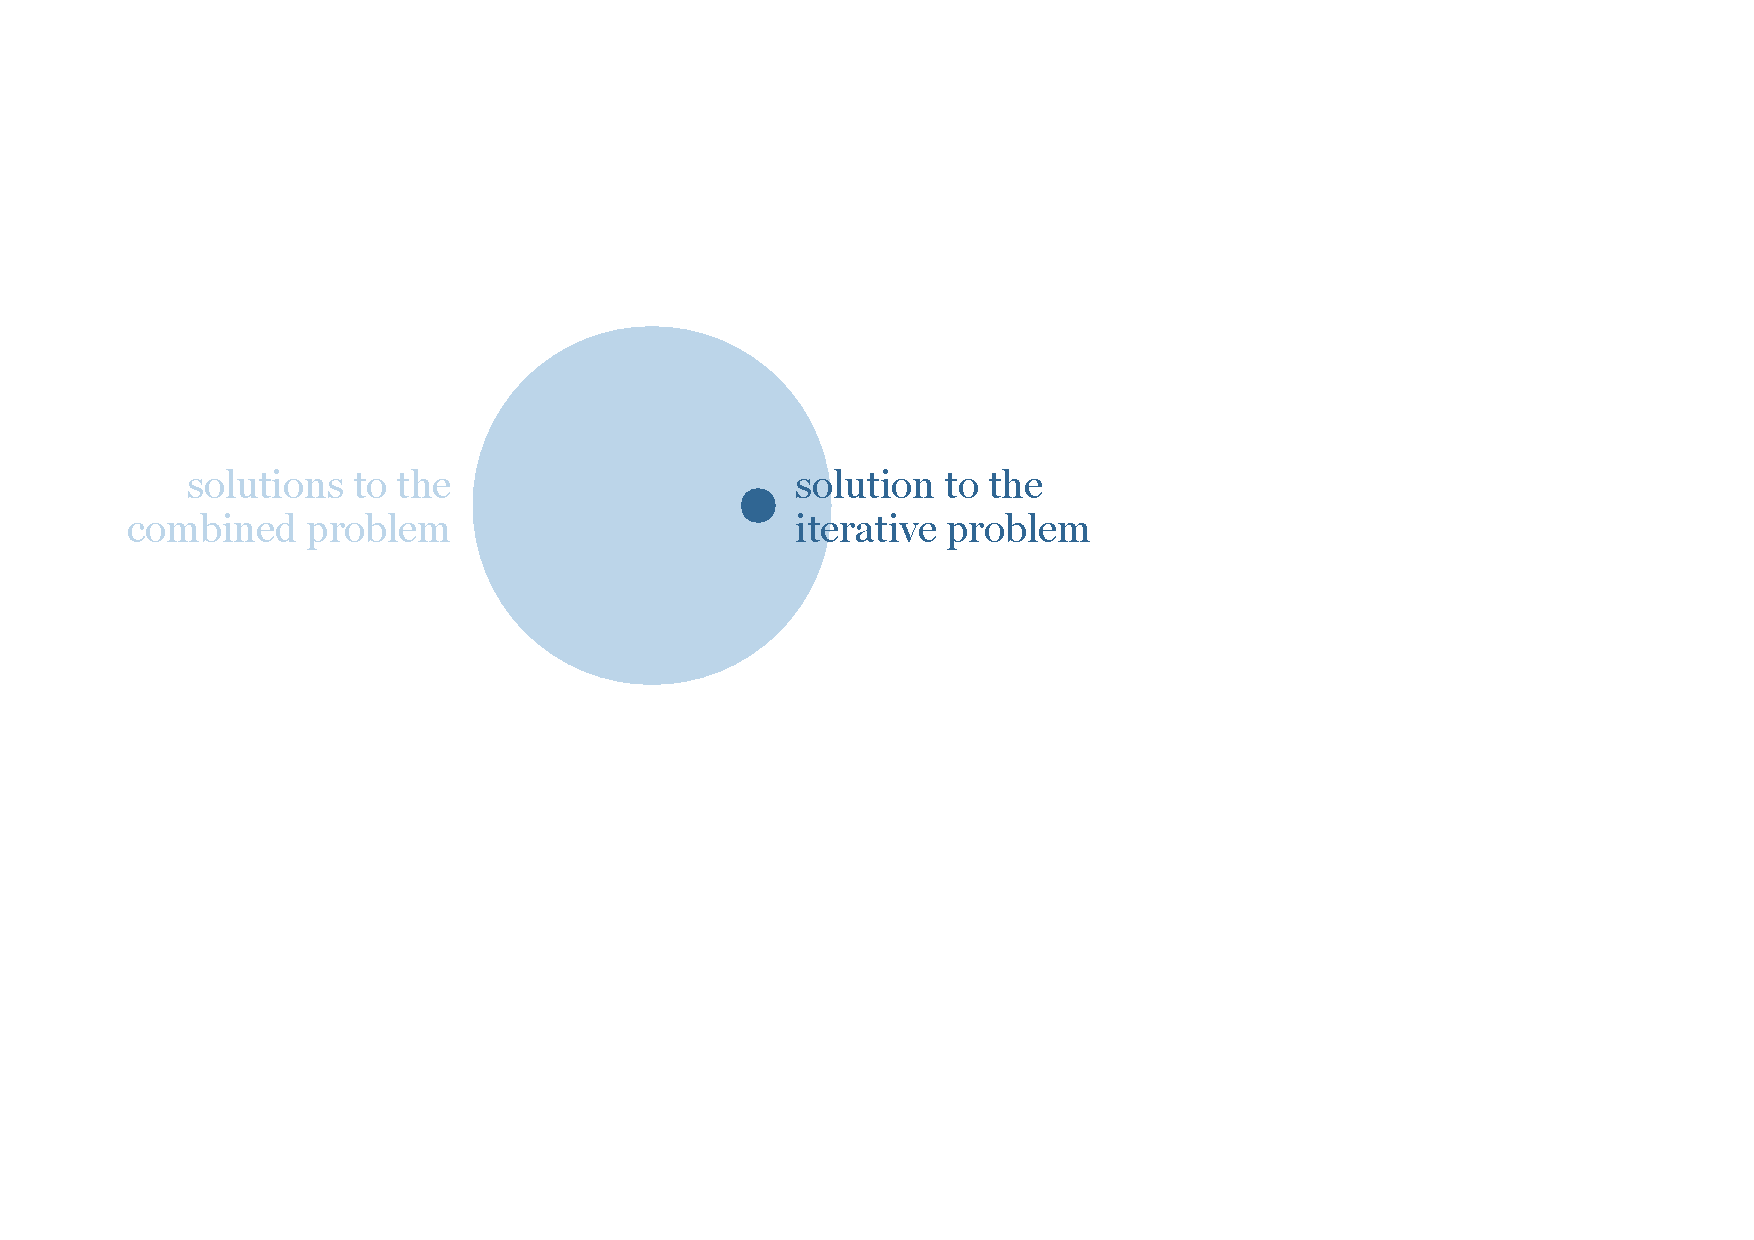
\includegraphics[width=1\textwidth]{./images/pca/venn.pdf}
	}
\end{figure}
%<figure class="narrow">
%<img src="/images/pca/venn.svg" />
%</figure>

These solutions are the same for both perspectives: variance maximization and reconstruction error minimization. We have two unresolved questions about this image.

First, how is it that the solution to the iterative problem (the PCA solution) reaches the same optimum as the solutions to the combined approach? Take a second to consider how strange this is. Solving the iterative problem is a greedy search: once we have chosen \(\rc{\mbw_1}\) we can't ever go back. The process for the combined approach solves all the vectors in sync. How is it that this ability to tune the vectors in concert doesn't give us any advantage in the optimum we find?

The second question, and the question we will answer first, is what is the meaning of the PCA solution among the combined solutions? How can we \emph{characterize} this solution?

The answer to the second question can be summarized in one phrase:

\begin{displayquote}
The principal components are \emph{eigenvectors}.
\end{displayquote}

\index{Eigenvector}

Depending on your background, this will raise one of two questions. \emph{The eigenvectors of what?} or, more simply \emph{What are eigenvectors?} Let's start with the second question, and work our way back to the first.

\subsection{What are eigenvectors?}

The most common, and probably the most intuitive way to think about matrices is \emph{as transformations of points in space}. If we have some vector \(\mbx\) and we multiply it by a matrix \(\bc{\mbA}\), we get a new point \(\mby = \bc{\mbA}\mbx\). If \(\bc{\mbA}\) is square, then \(\mbx\) and \(\mby\) are in the same space. 

\index{Matrix transformations}

A good way to visualize this is by \emph{domain coloring}. We take a large number of points, arranged in a grid, and we color them by some image. This could be a simple color gradient, but we can also choose a photograph or some other image.  Following \href{https://en.wikipedia.org/wiki/Eigenvalues_and_eigenvectors}{Wikipedia's example}, we'll use a picture of the Mona Lisa.

\index{Domain coloring}\index{Mona Lisa}

\begin{figure}[H]
	\centerline{
	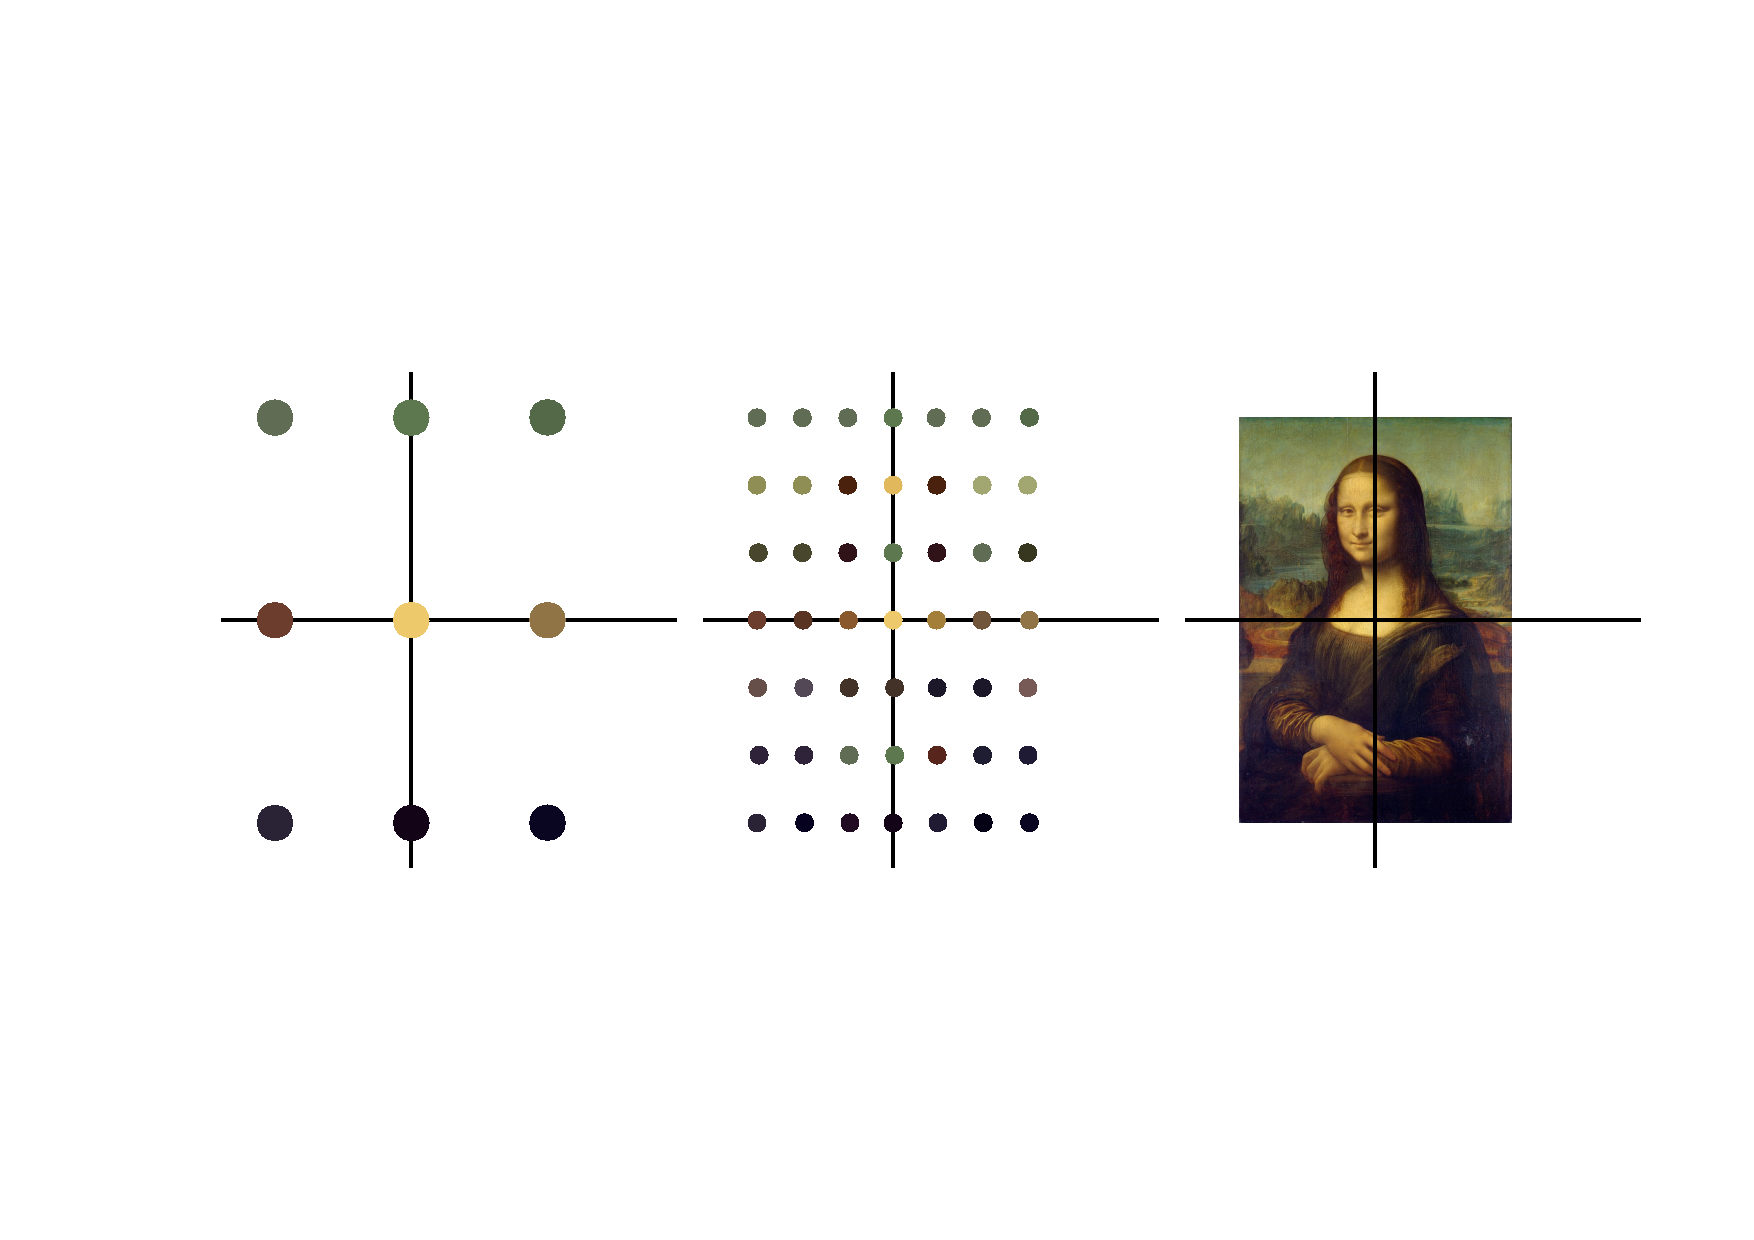
\includegraphics[width=0.7\textwidth]{./images/pca/domain-coloring.pdf}
	}
	\caption*{An increasingly fine-grained domain coloring using the Mona Lisa.}
\end{figure}
%<figure class="narrow">
%<img src="/images/pca/domain-coloring.svg" />
%<figcaption>An increasingly fine-grained domain coloring using the Mona Lisa.</figcaption>
%</figure>

If we apply the transformation \(\bc{\mbA}\) to each of these points, we can tell what effect the matrix has on this space. 

\begin{figure}[H]
	\centerline{
	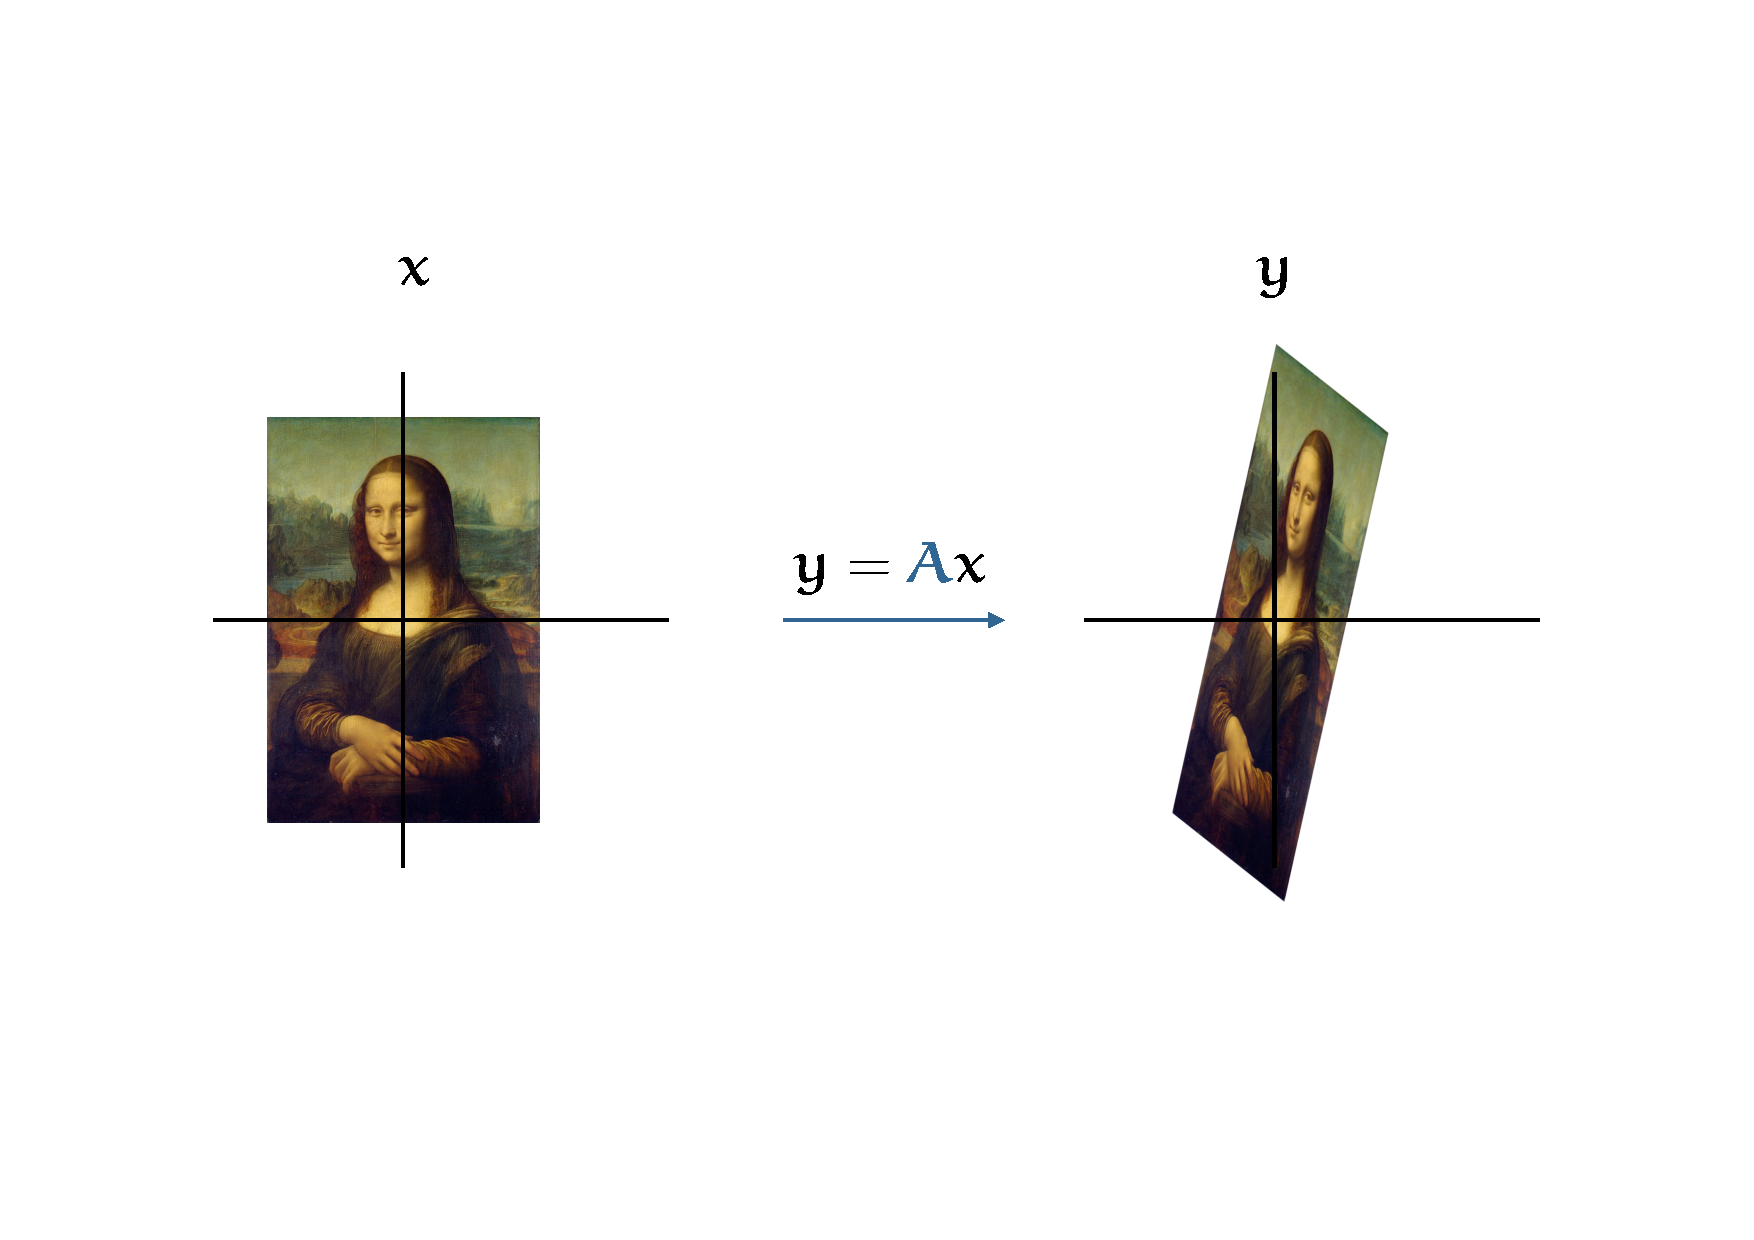
\includegraphics[width=1\textwidth]{./images/pca/basic-transform.pdf}
	}
\end{figure}

%<figure class="narrow">
%<img src="/images/pca/basic-transform.svg" />
%</figure>

All the points are mapped to a new position by \(\bc{\mbA}\) and poor Lisa ends up squished and stretched in various directions. Transformations expressible in a matrix are linear transformations. These are the transformations for which a line in the original image is still a line in the transformed image. This means that we can rotate, stretch, squish and flip the image in any direction we like, but we can't warp, bend or tear it.

In this language of transformation, we can very naturally define what eigenvectors are. The \textbf{eigenvectors of a square matrix \(\bc{\mbA}\)} are defined as those vectors (i.e. points in the image) for which the \emph{direction} doesn't change under transformation  by \(\bc{\mbA}\).

\index{Eigenvector}

It's simplest to see what this looks like for a \emph{diagonal matrix}. For instance in the transformation

\[
\mby = \bc{\begin{pmatrix}2 & 0 \\ 0 & \tfrac{1}{2}\\\end{pmatrix}}\mbx
\]
%
the matrix acts independently on the first and second dimensions, squishing one, and stretching the other.

\begin{figure}[H]
	\centerline{
	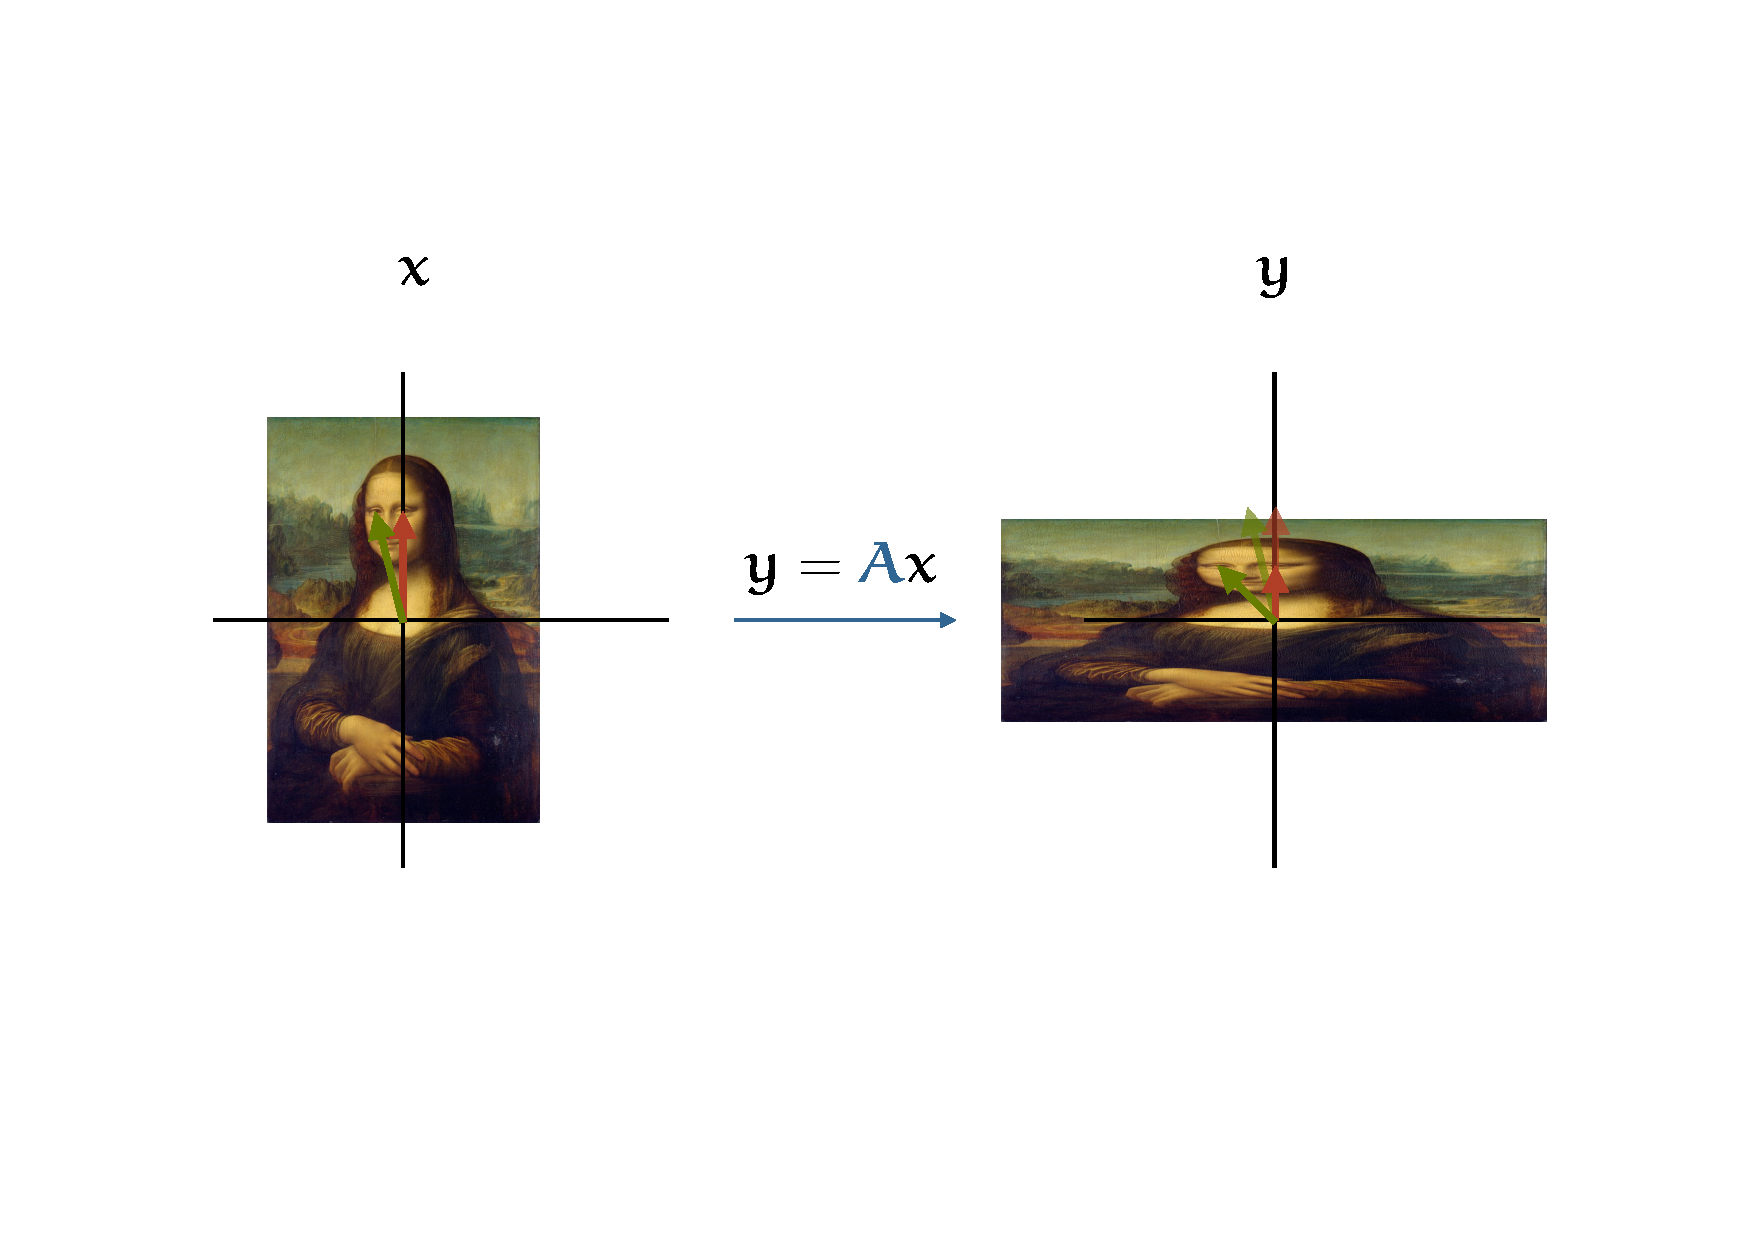
\includegraphics[width=1.2\textwidth]{./images/pca/diagonal.pdf}
	}
\end{figure}

%<figure class="narrow">
%<img src="/images/pca/diagonal.svg" />
%</figure>

In this image we've also drawn two vectors: one \gc{to the middle of Mona Lisa's left eye}, and one \rc{to middle of the right}. Since Leonardo put the right eye dead center in the painting (not by accident, I imagine), the red vector shrinks, but doesn't change direction. The green vector is affected by both the squishing and the stretching, so its direction and magnitude both change. Hence, the red vector is an eigenvector, and the green vector isn't.

In a diagonal matrix, the eigenvectors are always the vectors that point in the same directions as the axes, so they're easy to identify. In general square matrices, finding the eigenvectors is more tricky. 

\index{Eigenvector!of a diagonal matrix}

\begin{aside}See if you can find an eigenvector for the first transformation, shown above. One trick is to start with a random vector, and if it changes direction, transplant it back to the untransformed image and iterate until the vector doesn't change anymore.
\end{aside}

Formally, a vector \(\rc{\mbv}\) is an eigenvector of \(\bc{\mbA}\) if the following holds for some scalar \(\bc{\lambda}\):

\[
\bc{\mbA}\rc{\mbv} = \bc{\lambda}\rc{\mbv} \p
\]

\index{Eigenvector!definition}

This is just a symbolic version of what we said in words above: if \(\rc{\mbv}\) is an eigenvector of \(\bc{\mbA}\), then transforming it changes its magnitude but not its direction, which is the same as saying we can multiply it by a scalar instead of by a matrix. The scalar corresponding to the eigenvector, in this case \(\bc{\lambda}\) is called an \textbf{eigenvalue} of the matrix.

\begin{aside}It's not at all clear from the definition why these vectors should be meaningful or special. For now, just trust me that eigenvectors are worth knowing about.
\end{aside}

To build your intuition, consider for a second the question of whether a pure rotation matrix has eigenvectors (the zero vector doesn't count). It shouldn't take long to convince yourself that a rotation in two dimensions doesn't. At least, not usually. There are two exceptions: rotating by 360 degrees (which is just \(\mbI\)) and rotating by 180 degrees. In both cases, every vector is an eigenvector. In the first with eigenvalue \(\bc{1}\), and  in the second with eigenvalue \(\bc{-1}\). 

\index{Eigenvector!of a rotation matrix}

In three dimensions, rotation is a different story: try pointing straight up in the air and spinning around. The direction of your arm doesn't change as you rotate, so your arm is an eigenvector. Your nose does change direction, so your nose is not an eigenvector.

We saw that when a matrix is diagonal, its eigenvectors are \emph{aligned with the axes}, so they're easy to find. For other matrices, we need to do some more work. One trick is to simply transform the matrix so that the eigenvectors are aligned with the axes, and then to transform it back again.

This is easiest to understand if we work backwards: given some eigenvectors, find the transformation for them.

Here are some vectors drawn on top of the Mona Lisa. What is the transformation for which these vectors do not change direction? 


\begin{figure}[H]
	\centerline{
	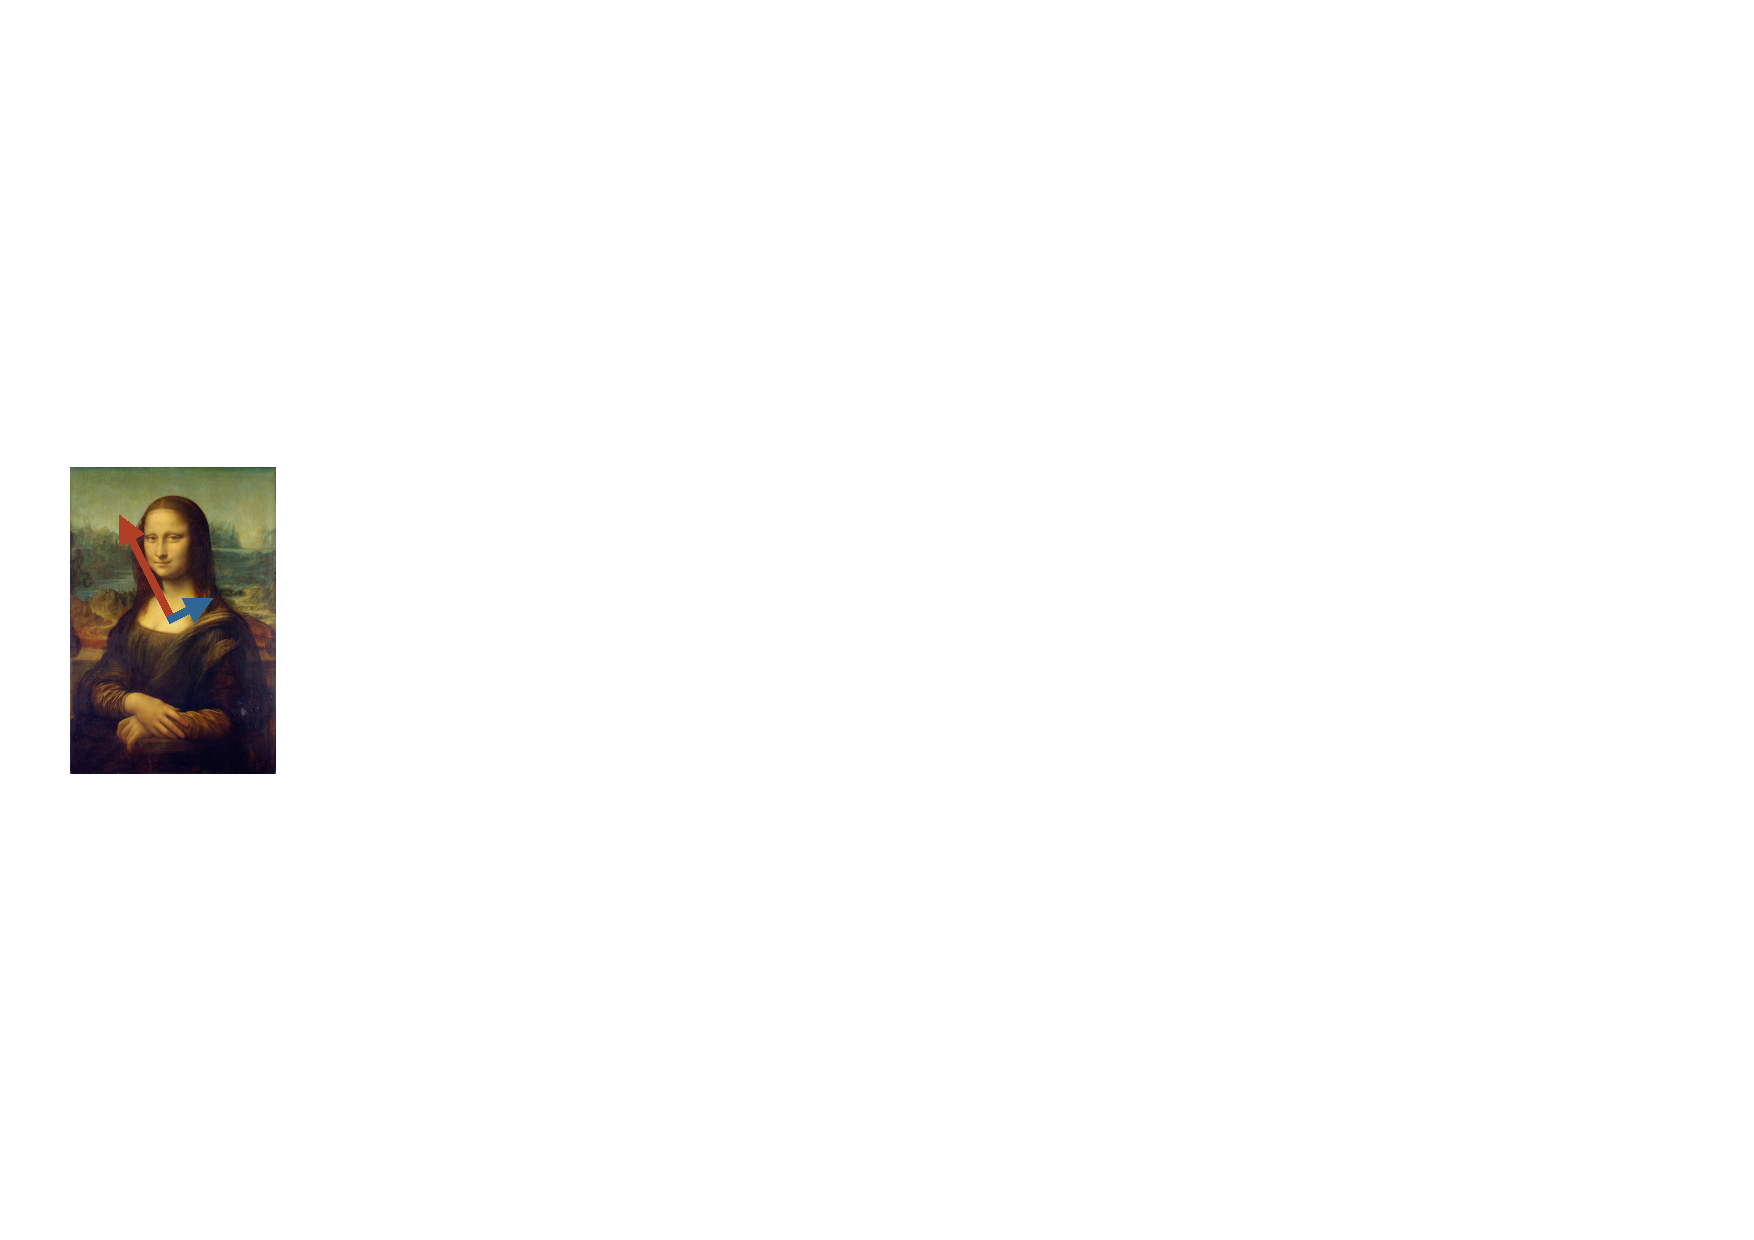
\includegraphics[width=.6\textwidth]{./images/pca/mona-eigen.pdf}
	}
\end{figure}

%<figure class="narrow centering">
%<img src="/images/pca/mona-eigen.svg" class="own-size"/>
%</figure>

We have made things easy for ourselves by making the eigenvectors orthogonal. This means we can \emph{rotate} the image to put the eigenvectors on the axes. We can then do any stretching and squishing we like along the axes, and rotate the image back. 

\begin{figure}[H]
	\centerline{
	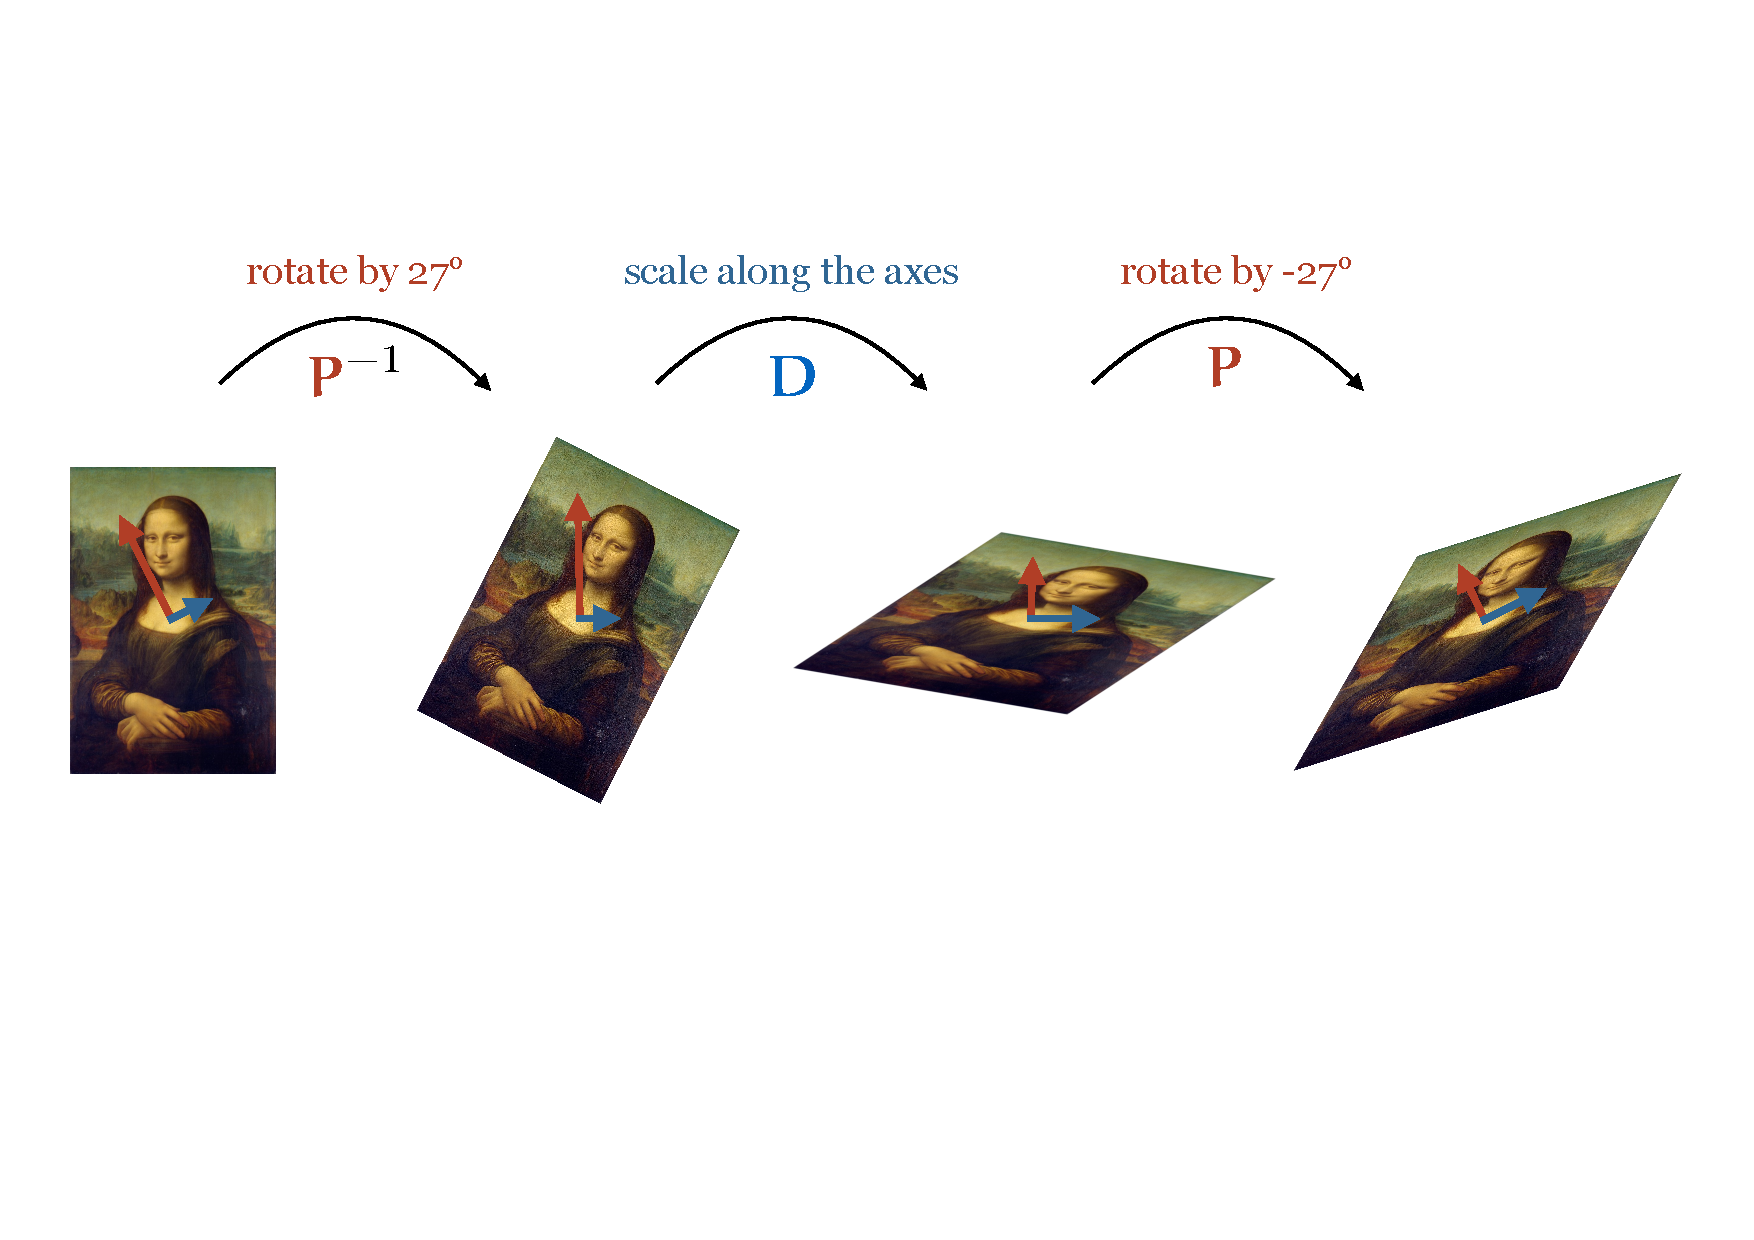
\includegraphics[width=1.2\textwidth]{./images/pca/mona-steps.pdf}
	}
\end{figure}

%<figure class="narrow">
%<img src="/images/pca/mona-steps.svg"/>
%</figure>

Note how, comparing the first and the last image, the red and blue vector change their shape, but not their direction.

Any change we make to the direction of the vectors in the \rc{first step} is reversed exactly in the \rc{last step}: the only permanent change to any \emph{directions} is made in the \bc{middle step}. Therefore, those vectors which don't change direction in the middle step, never change direction at all, and must therefore be eigenvectors. These are the vectors that align with the axes in the middle figure, since the middle transformation is along the axes. Therefore, the vectors which are mapped to align with the axes by the first step are the eigenvectors of the complete transformation \emph{consisting of all three steps}.

All three of these steps can be expressed as matrix transformations. We will call the matrix for the \rc{last step} \(\rc{\mbP}\). The \rc{first step} is then \(\rc{\mbP}^{-1}\), since it needs to undo \(\rc{\mbP}\) exactly. This means that we must require that \(\rc{\mbP}\) is invertible. 

\begin{aside}We could also call the first step \(\rc{\mbP}\) and the last step \(\rc{\mbP}^{-1}\), of course, but it works out more neatly if we call the last step \(\rc{\mbP}\).\end{aside}

In the example, \(\rc{\mbP}\) is a rotation matrix, but the principle generalizes to all invertable matrices. 

We have seen the approach for the middle step already: it is expressed by a diagonal matrix, which we'll call \(\bc{\mbD}\). The composition of these three steps is our transformation matrix \(\bc{\mbA}\). 

\pagebreak

\noindent We compose transformations by multiplying their matrices, so we have:

\[
\bc{\mbA} = \rc{\mbP}\bc{\mbD}\rc{\mbP}^{-1} 
\]

Note that for a transformation \(\bc{\mbA}\mbx = \rc{\mbP}\bc{\mbD}\rc{\mbP}^{-1}\mbx\), the rightmost matrix is applied first, so the direction of the matrices is reversed from the steps in  image above.

Now we can work backwards: For any given matrix \(\bc{\mbA}\), \emph{if} we can decompose it in this way, as the product of some \rc{invertible matrix}, some \bc{diagonal matrix} and the \rc{inverse of the invertable matrix}, then we know three things:

\begin{itemize}
\item The eigenvectors of \(\bc{\mbA}\) are the vectors that are mapped by \(\rc{\mbP}^{-1}\) to align to the axes. Any change of direction introduced by \(\rc{\mbP}^{-1}\) is undone by \(\rc{\mbP}\), so the only vectors whose direction is unchanged are those mapped to the eigenvectors of \(\bc{\mbD}\) (i.e. to the axes).
\item The eigenvectors are also those vectors which to which axis-aligned vectors are transformed by \(\rc{\mbP}\).
\item The eigen\emph{values} of \(\bc{\mbA}\) are the elements along the diagonal of \(\bc{\mbD}\). Any change of magnitude introduced by \(\rc{\mbP}^{-1}\) is undone by \(\rc{\mbP}\), so only the changes made by \(\bc{\mbD}\) remain. An eigenvector mapped to axis \(i\) by \(\rc{\mbP}\) is scaled by \(\bc{D}_{ii}\), which is therefore the corresponding eigenvalue.
\end{itemize}


For a given matrix \(\bc{\mbA}\), finding a diagonal matrix \(\bc{\mbD}\) and an invertible matrix \(\rc{\mbP}\) so that \(\bc{\mbA} = \rc{\mbP}\bc{\mbD}\rc{\mbP}^{-1}\) is called a \textbf{diagonalization} or an \textbf{eigendecomposition} of \(\bc{\mbA}\). 

\index{Diagonalization}\index{Eigendecomposition}

So, given a diagonalization of \(\bc{\mbA}\), which are the eigenvectors? We use the second bullet point above. If we take an axis-aligned vector and transform it by \(\rc{\mbP}\), the result is an eigenvector.

We have one eigenvalue per axis, so we'll look for one eigenvector for each. For the vectors to feed to the transformation, we can just take axis-aligned unit vectors (also known as one-hot vectors). Each will transform to an eigenvector. We can do the transformation for all vectors in one go by concatenating the vectors as the columns of one matrix. For the unit vectors this simply results in the identity matrix \(\mbI\), and for the eigenvectors, this results in a matrix we will call \(\oc{\mbE}\). So we are looking the matrix \(\oc{\mbE}\) for which 


\index{One-hot vector}\index{Axis-aligned vector}

\[
\rc{\mbP}\mbI = \oc{\mbE} \p
\]

Removing \(\mbI\) tells us that the eigenvectors we are looking for are simply the columns of \(\rc{\mbP}\).

\subsection{The spectral theorem}

Note that we were careful above to say \emph{if} \(\bc{\mbA}\) can be diagonalized. Not all square matrices can be diagonalized. A theorem showing if and when a particular class of transformations can be diagonalized is called a \emph{spectral theorem}.

\index{Spectral theorem}

\begin{aside}The set of eigenvalues of a matrix is sometimes called its spectrum, so methods and results using these principles often use the adjective \emph{spectral}. For instance, we have \href{https://en.wikipedia.org/wiki/Spectral\_clustering}{spectral clustering}, \href{https://en.wikipedia.org/wiki/Spectral\_graph_theory}{spectral graph theory} and \href{https://en.wikipedia.org/wiki/Spectral\_method}{spectral ODE solvers}.
\end{aside}

\index{Spectral methods}\index{Spectrum (of a matrix)}

There are many spectral theorems, but we'll only need the simplest. The spectral theorem for \emph{symmetric matrices}. A symmetric matrix is a square matrix \(\bc{\mbA}\) which is symmetric across the diagonal. That is, it has \(\bc{A}_{ij} = \bc{A}_{ji}\), or equivalently \(\bc{\mbA}^T = \bc{\mbA}\). We'll call this \emph{the} spectral theorem in the context of this book.

To state the theorem, we first need to define \textbf{orthogonal matrices}. These are square matrices in which all columns are mutually orthogonal unit vectors. 

\index{Orthogonal matrix}

This should sound familiar, it's the constraint we placed on our principal components in the previous chapter. In the combined problem, the constraint \(\rc{\mbW}^T\rc{\mbW} = \mbI\) is simply a requirement that the matrix \(\rc{\mbW}\) be orthogonal.

Why? Remember that matrix multiplication is just a collection of all dot products of rows on the left with columns on the right, so in this case all columns of \(\rc{\mbW}\) with all other columns of \(\rc{\mbW}\). On the diagonal of \(\rc{\mbW}^T\rc{\mbW}\), we find all dot products of columns of \(\rc{\mbW}\) with themselves, which are all \(1\), because they are all unit vectors. Off the diagonal we find all dot products of all columns with other columns. These are all zero, because they are all mutually orthogonal.

\begin{aside}Geometrically, orthogonal matrices represent those transformations that do not change the magnitude of any vector: that is, rotations and reflections.
\end{aside}

A very useful property of orthogonal matrices is that their inverse is equal to their transpose: \(\rc{\mbW}^{-1} = \rc{\mbW}^T\). This follows directly from the fact that \(\rc{\mbW}^T\rc{\mbW} = \mbI\), because the inverse of \(\rc{\mbW}\) is defined as a matrix \(\rc{\mbW}^{-1}\) such that \(\rc{\mbW}^{-1}\rc{\mbW} = \mbI\).

\index{Orthogonal matrix!inverse of}

This property makes orthogonal matrices especially nice to work with, since we can take the inverse---usually a costly and numerically unstable operation---by flipping the indices around, which we can do in constant time, with no numerical instability. 

We can now state the spectral theorem.

\begin{theorem}[The spectral theorem.] Call a matrix \(\bc{\mbA}\) \emph{orthogonally diagonalizable} if it is diagonalizable  with the additional constraint that \(\rc{\mbP}\) is orthogonal
\[
\bc{\mbA} = \rc{\mbP}\bc{\mbD}\rc{\mbP}^T \p
\]

A matrix \(\bc{\mbA}\) is orthogonally diagonalizable if and only if \(\bc{\mbA}\) is symmetric.
\end{theorem}

\index{Spectral theorem!statement}

Proving this now would require us to discuss too many extra concepts that aren't relevant for this part of the story. On the other hand, this theorem is very much the heart of PCA: everything it is and can do follows from this result. We'll take it at face value for now, and answer the rest of our questions. The next chapter will be entirely dedicated to proving the spectral theorem.

For now, just remember that if we have a square, symmetric matrix, we can diagonalize it with an orthogonal matrix \(\rc{\mbP}\) and a diagonal matrix \(\bc{\mbD}\). The diagonal elements of \(\bc{\mbD}\) will be the eigenvalues and the columns of \(\rc{\mbP}\) will be the corresponding eigenvectors. 

Note that the spectral theorem implies that there are \(\gc{n}\) eigenvalues (since \(\bc{\mbD}\) has \(\gc{n}\) diagonal values). Some of them might be zero, but we need not worry about that at the moment. In upcoming chapters, we'll develop some concepts that help us characterize what it means for eigenvalues to be zero.

Finally, notice that for any such diagonalization, we can shuffle the eigenvalues around and get another diagonalization (we just have to shuffle the columns of \(\rc{\mbP}\) in the same way). Since the ordering of the eigenvalues in \(\bc{\mbD}\) is arbitrary, we usually sort the from largest to smallest, calling the largest the \textbf{first eigenvector} and the smallest the \textbf{last eigenvector}. As you may expect, we'll see later that these match the ordering of the principal components. We'll call the decomposition with the eigenvectors ordered like this, the \emph{canonical} orthogonal diagonalization.

\index{Eigenvectors!ordering of}\index{Canonical orthogonal diagonalization}

\subsection{The eigenvectors of which matrix?}

Let's get back to the PCA setting. Where do we find eigenvectors in this picture? We have a matrix, the data matrix \(\mbX\), but it isn't square, and it's never used as a transformation. 

In fact, the eigenvectors that end up as the principal components are the eigenvectors of the \emph{covariance matrix} of our data \(\mbX\).

\begin{displayquote}
The principal components are the eigenvectors \bc{of the covariance matrix}.
\end{displayquote}

Let's start by reviewing what a covariance matrix is. When we talk about one-dimensional data, we often discuss the variance: a measure for how spread out the numbers are. We can think of this as a measure of \emph{predictability}. The more spread out the points are, the more difficult it is to predict where a randomly sampled point might be. If the variance is very small, we know any point is very likely to be near the mean of the data. If it's very large, we are less sure.

\index{Covariance matrix}

The covariance matrix is the analogue to this for \(\bc{m}\)-dimensional data, like our dataset \(\mbX\). It tells us not just how spread out the points are along the axes (the variance of each feature) but also how spread out the points of one feature are, \emph{given the value of another feature}. 

\pagebreak

\noindent Consider the following 2D dataset:

\begin{figure}[H]
	\centerline{
	\includesvg[width=1\textwidth]{./images/pca/covariance.svg}
	}
\end{figure}

%<figure class="narrow centering">
%<img src="/images/pca/covariance.svg" class="three-quarters"/>
%</figure>

The variance for both features is 1, so the data is pretty spread out. It has high variance, and is therefore relatively unpredictable. However, if I know the value of feature 1, suddenly the likely values of feature 2 become much narrower. 

This is because the data has high \emph{co}variance between the two features: knowing the value of one, tells us a lot about the value of another. Another way of saying this is that the two features are highly \emph{correlated}. Here are the different ways data can be \emph{linearly} correlated in 2D.

\begin{figure}[H]
	\centerline{
	\includesvg[width=1.1\textwidth]{./images/pca/covs-3.svg}
	}
\caption*{Three ways data can be correlated. The bottom row shows the covariance matrices of each dataset (explained below).}
\end{figure}

%<figure class="narrow">
%<img src="/images/pca/covs-3.svg" />
%<figcaption>Three ways data can be correlated. The bottom row shows the covariance matrices of each dataset (explained below).
%</figcaption>
%</figure>

Pay particular attention to the middle example: perfectly \emph{decorrelated} data. In such data, the features are independent: knowing the value of one tells us nothing about the value of the other. This is an important property of good \emph{latent features}. For instance, in the Olivetti data from the last  chapter, many of the observed features (the pixel values) were highly correlated, but the latent features we extracted by PCA (the gender, the age, the lighting) were largely decorrelated. If the data is not biased, knowing the age of a subject shouldn't tell you anything about the way they were lit or how feminine they appear.

The formula for the variance of feature \(\bc{j}\), as we've seen before, is 

\[
\text{Var}_\mbX(\bc{j}) = \kc{\frac{1}{n}} \sum_\gc{i} (\bar x_\bc{j} - X_{\gc{i}\bc{j}})^2
\]

\index{Variance}

Where \(\bar x_\bc{j}\) is the mean of feature \(\bc{j}\), which is \(0\) if the data is mean-centered. The \emph{co}variance between features \(\bc{j}\) and \(\bc{k}\) is defined as

\[
\text{Cov}_\mbX(\bc{j}, \bc{k}) = \kc{\frac{1}{n}} \sum_\gc{i} (\bar x_\bc{j} - X_{\gc{i}\bc{j}})(\bar x_\bc{k} - X_{\gc{i}\bc{k}})
\]

\index{Covariance!definition}

\begin{aside}These are both \emph{estimates}. The distribution from which the data was sampled has some invisible (co)variance, which we estimate from the data by these formulas. For a maximum likelihood estimate, we divide by \(\kc{n}\), for an unbiased estimate by \(\kc{n-1}\). For large data, the difference is negligible, so I'll use the first to keep the formulas simple.
\end{aside}

For mean-centered data, these simplify to

\begin{align*}
\text{Var}_\mbX(\bc{j}) &= \kc{\frac{1}{n}} \sum_\gc{i} X_{\gc{i}\bc{j}} X_{\gc{i}\bc{j}}\\
\text{Cov}_\mbX(\bc{j}, \bc{k}) &= \kc{\frac{1}{n}} \sum_\gc{i} X_{\gc{i}\bc{j}} X_{\gc{i}\bc{k}} \p
\end{align*}

Note two things about these equations:
\begin{enumerate}
\item The variance is just the covariance of a feature \emph{with itself}: \(\text{Var}_\mbX(\bc{j}) = \text{Cov}_\mbX(\bc{j}, \bc{j})\).
\item If we ignore the multiplier \(\kc{\tfrac{1}{n}}\), the covariance is the dot product of one column of \(\mbX\) with another.
\end{enumerate}

This means that if we make a \bc{big matrix} with all covariances between features \(\bc{j}\) and \(\bc{k}\), we can compute that matrix by a simple matrix multiplication:

\[
\text{Cov}(\mbX) = \kc{\frac{1}{n}}\mbX^T\mbX
\]

\index{Covariance!as a matrix}

\begin{figure}[H]
	\centerline{
	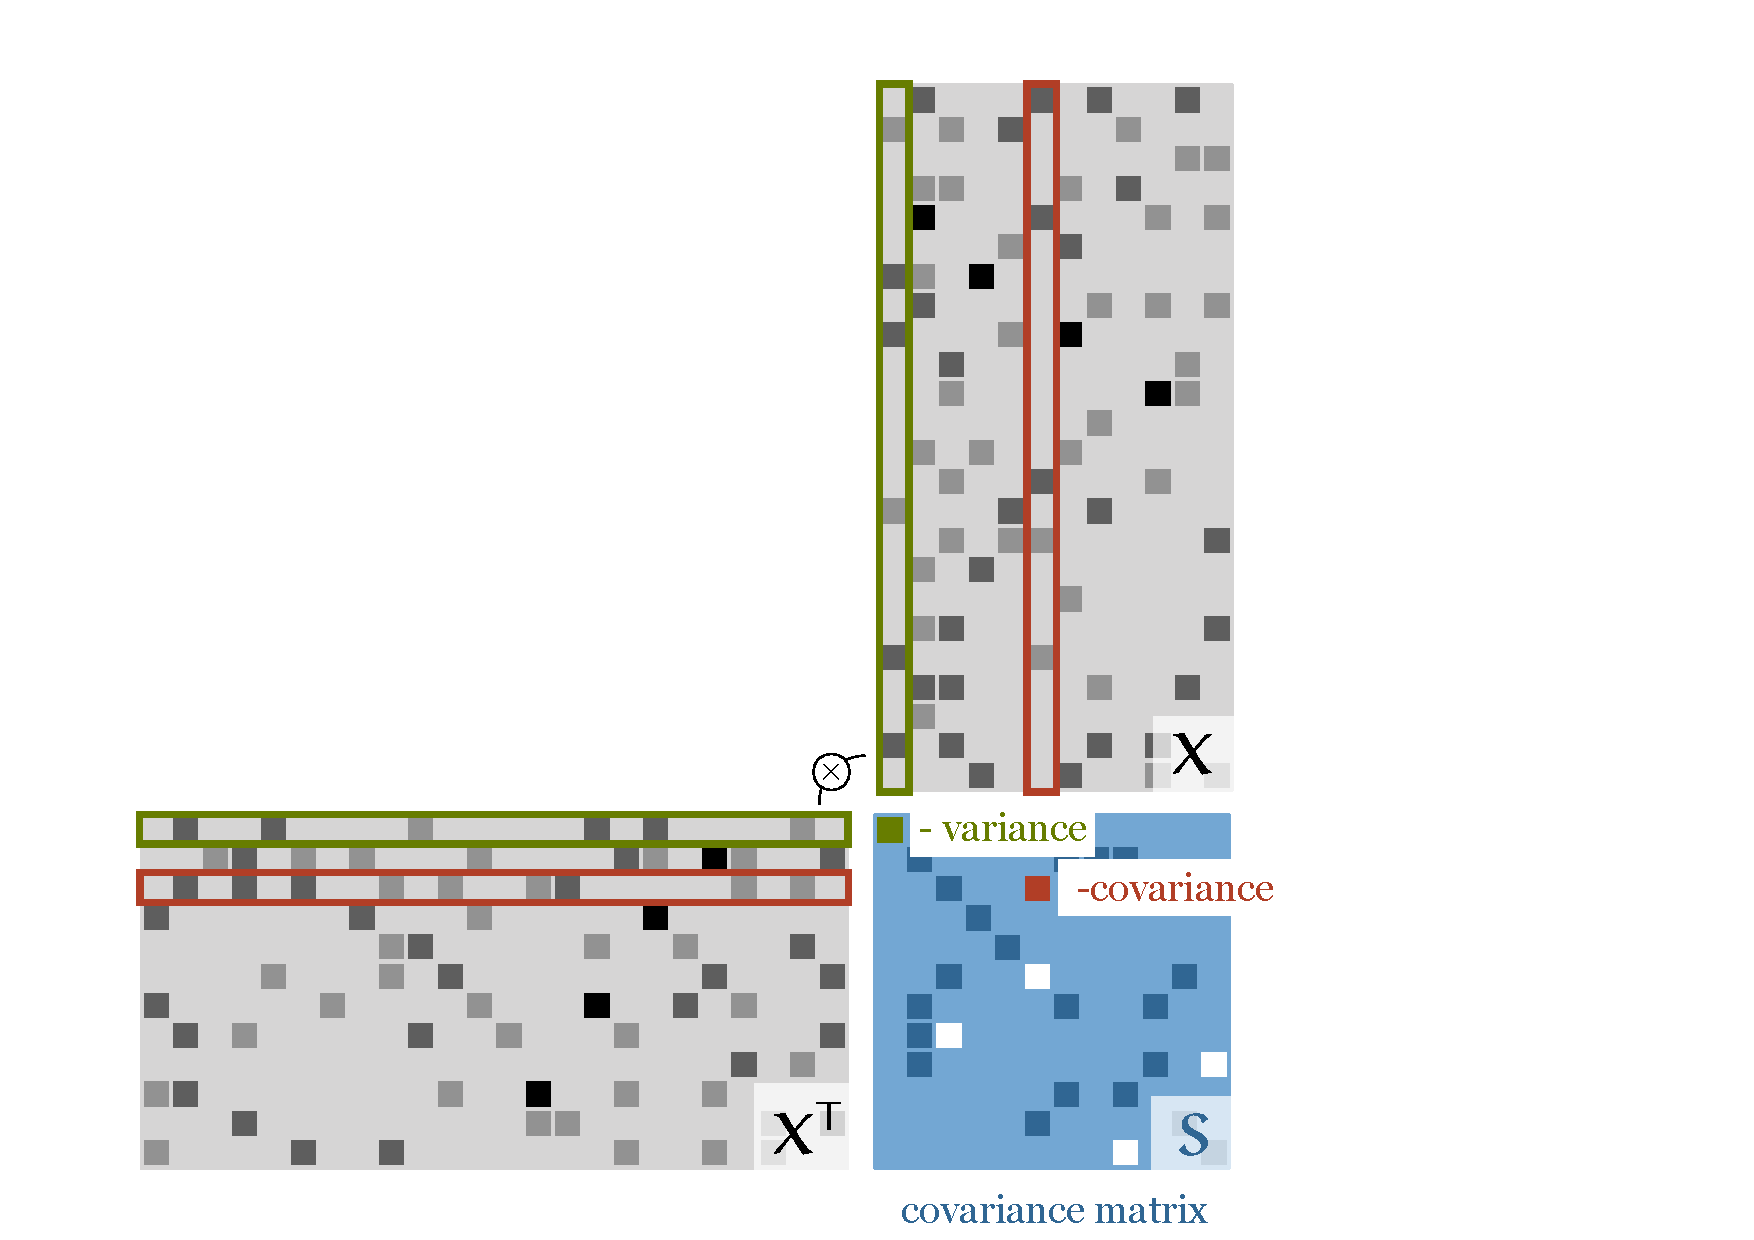
\includegraphics[width=1\textwidth]{./images/pca/covmult.pdf}
	}
\end{figure}

%<figure class="narrow">
%<img src="/images/pca/covmult.svg" class="three-quarters"/>
%</figure>
%
This matrix is symmetric, since \(\text{Cov}(\bc{j}, \bc{k}) = \text{Cov}(\bc{k}, \bc{j})\), and it has the variances of the various features along the diagonal. 

\begin{aside}For any matrix, \(\mbX\) of any size, \(\bc{\mbM} = \mbX^T\mbX\) is square and symmetric: \(\bc{M}_{ij} = \bc{M}_{ij}\) because both values are the dot product of columns \(i\) and \(j\) in the data.
\end{aside}

We'll denote the covariance matrix of our dataset \(\mbX\) by \(\bc{\mbS}\) . This is the matrix that we're interested in: the eigenvectors of \(\bc{\mbS}\) coincide with the principal components of \(\mbX\).

I expect that that doesn't immediately make a lot of intuitive sense. We've developed eigenvectors in terms of matrices that transform points in space. We don't usually think of \(\bc{\mbS}\) as transforming space. It's not common to see a vector multiplied by \(\bc{\mbS}\). Yet, we can easily diagonalize \(\bc{\mbS}\). In fact, since it's symmetric, \gc{the spectral theorem} tells us that we can diagonalize it with an orthogonal matrix, and we can be sure that it has \(\gc{n}\) eigenvalues.

To develop some intuition for what these eigenvalues \emph{mean} we can have a look at the common practice of \textbf{data normalization}.

\section{Data normalization and basis transformations}

Data normalization is a very common data pre-processing step in many data science processes. For many applications we don't much care about the natural scale of the data, and we instead want the data to lie in a predictable range. For one-dimensional data, one way to do this is to rescale the data so that its mean equals \(0\), and its variance equals \(1\). We achieve this easily by first shifting the data so that the mean is at \(0\), and then scaling uniformly until the variance is \(1\).

\index{Normalization}

To work out how to make this transformation, we can imagine that our data \emph{originally} had mean \(0\), and variance \(1\), and was then transformed by scaling and then adding some constant value. That is, every point \(x\) we observed was derived from an unseen point \(z\) by two parameters \(\bc{s}\) and \(\oc{t}\) as 

\[
x = \bc{s}z + \oc{t}
\]

with the \(z\)'s having mean \(0\) and variance \(1\). We will call \(z\) the \textbf{hidden} or \textbf{latent} variable behind the \textbf{observed variable} \(x\).

\index{Latent variable}\index{Hidden variable}\index{Observed variable}

After scaling by \(\bc{s}\), the mean of the "original" data is still \(0\), so we should set \(\oc{t} = \bar x\) to end up with the correct mean for our observed data. To work out \(\bc{s}\), we move this term to the other side:

\[
x - \oc{\bar x} = \bc{s}z \p
\]

The left-hand side is the mean-centered data, and the right hand side is a scaled version of the latent data. Since variance isn't affected by the additive term, we get

\[
\text{Var}(\{x\}) = \kc{\frac{1}{n}}\sum_{z}(\bc{s}z)^2 = \bc{s}^2\kc{\frac{1}{n}}\sum_z z^2 = \bc{s}^2 \times \text{Var}(\{z\}) = \bc{s}^2 
\]

So, to end up with the correct variance for \(x\), we should set the \emph{square} of \(\bc{s}\) equal to the data variance, or equivalently, we should set \(\bc{s}\) equal to the data standard deviation \(\bc{\sigma}\) (the square root of the variance). So, the correct normalization is:

\[
x' = \frac{x - \oc{\bar x}}{\bc{\sigma}} \p
\]

\begin{aside}%
This may seem like an overly elaborate way to derive a pretty intuitive normalization, but we will generalize this approach to higher dimensions later, so it pays to understand the steps. 
\end{aside}

Instead of thinking of this operation as moving the data around, we can also think about it as keeping the data where it is, but just expressing it in different \emph{axes}. We move the origin to coincide with the data mean, and then scale \emph{the unit} (the length of the arrow from \(0\) to \(1\)) so that its tip lies at the point \(\oc{\bar x} + \bc{\sigma}\). On this new axis, the data is normalized.

\begin{figure}[H]
	\centerline{
	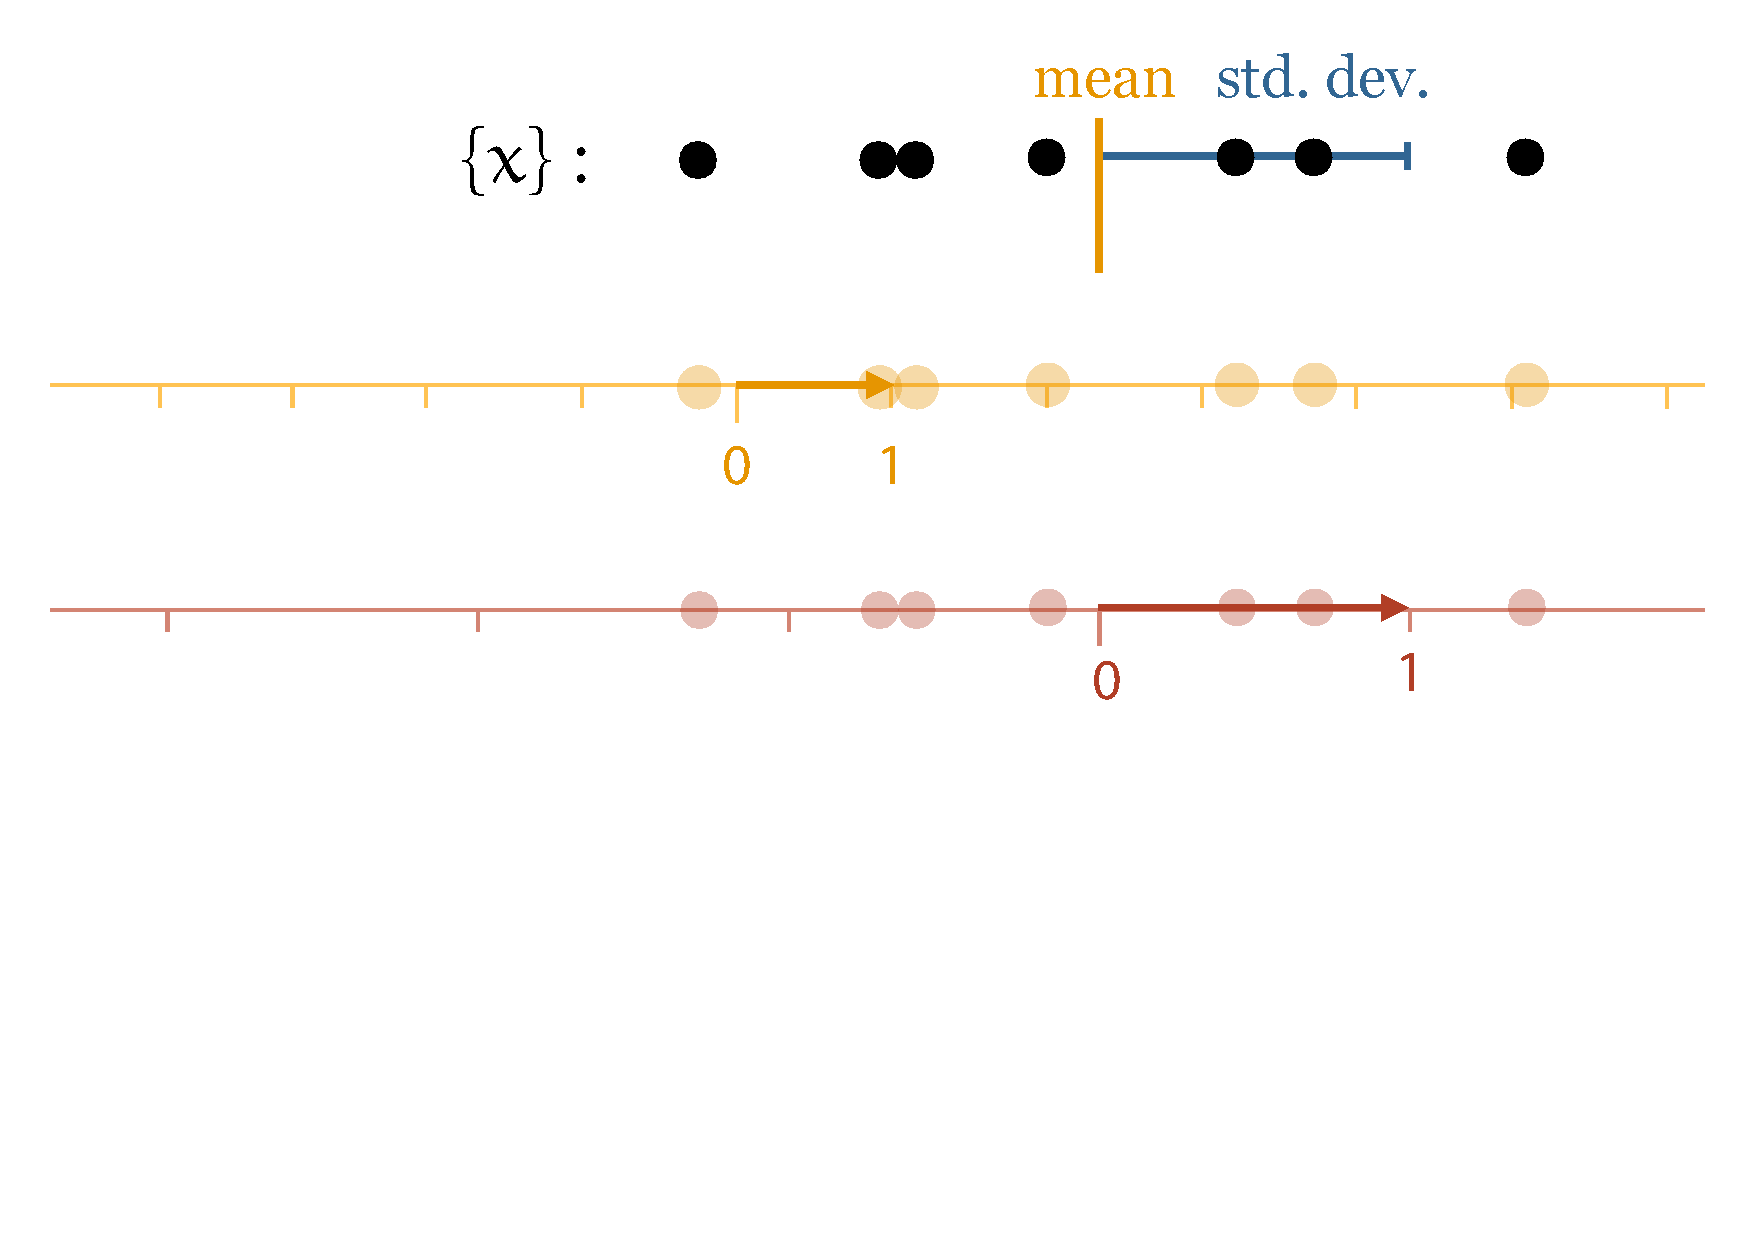
\includegraphics[width=1\textwidth]{./images/pca/onedbasis.pdf}
	}
	\caption*{We can see the operation of normalizing our one-dimensional data as simply expressing the same points on a \rc{different axis}. We change the location of the origin and the length of the unit, and our data is normalized.}
\end{figure}

%<figure class="narrow">
%<img src="/images/pca/onedbasis.svg"/>
%<figcaption>We can see the operation of normalizing our one-dimensional data as simply expressing the same points on a <span class="rc">different axis</span>. We change the location of the origin and the length of the unit (the arrow that points from \(0\) to \(1\)), and our data is normalized.
%</figcaption>
%</figure>
%
In higher dimensions, the \emph{units} we use to express points in space are often called a \emph{basis}. We take a bunch of vectors \(\rc{\mbb}_1, \ldots, \rc{\mbb}_k\), called the \emph{basis vectors} and express points as a sum of the basis vectors, each multiplied by a particular scalar, where the scalars are unique to the point we are expressing.

\begin{aside}Strictly speaking, for the set \(\rc{\mbb}_1, \ldots, \rc{\mbb}_k\) to be a basis, the vectors should also be \emph{linearly independent}. For our current purposes, we don't need to define this so precisely. We'll discuss linear independence in more detail in a later chapter.
\end{aside}

This is how our standard coordinate system works as well: in three dimensions, the basis vectors are \(\oc{\mbe}_1 = (1, 0, 0)\), \(\oc{\mbe}_2 = (0, 1, 0)\) and \(\oc{\mbe}_3 = (0, 0, 1)\). When we refer to a point \(\mbp\) with the coordinates (7, 3, 5), we are implicitly saying that 

\[
\mbp = 
7 \times \oc{\begin{pmatrix}1\\0\\0\end{pmatrix}} + 
3 \times \oc{\begin{pmatrix}0\\1\\0\end{pmatrix}} + 
5 \times \oc{\begin{pmatrix}0\\0\\1\end{pmatrix}}
\]

This is called the \textbf{standard basis}. It's a little elaborate for something so familiar, but it shows a principle we can apply for other sets of basis vectors. With any set of vectors \(\rc{B} = \{\rc{\mbb}_1, \ldots, \rc{\mbb}_k\}\), we can describe a point by writing down a vector \(\mbp^\rc{B}\), and computing

\index{Standard basis}\index{Basis!standard}

\[
\mbp = p_1^\rc{B} \rc{\mbb}_1 + \ldots + p_k^\rc{B} \rc{\mbb}_k 
\]

Here, \(\mbp\) are the coordinates of the point in the \oc{standard basis}, and \(\mbp^\rc{B}\) are the coordinates in the basis \(\rc{B}\).

\vspace{0.5em}
\begin{figure}[H]
	\centerline{
	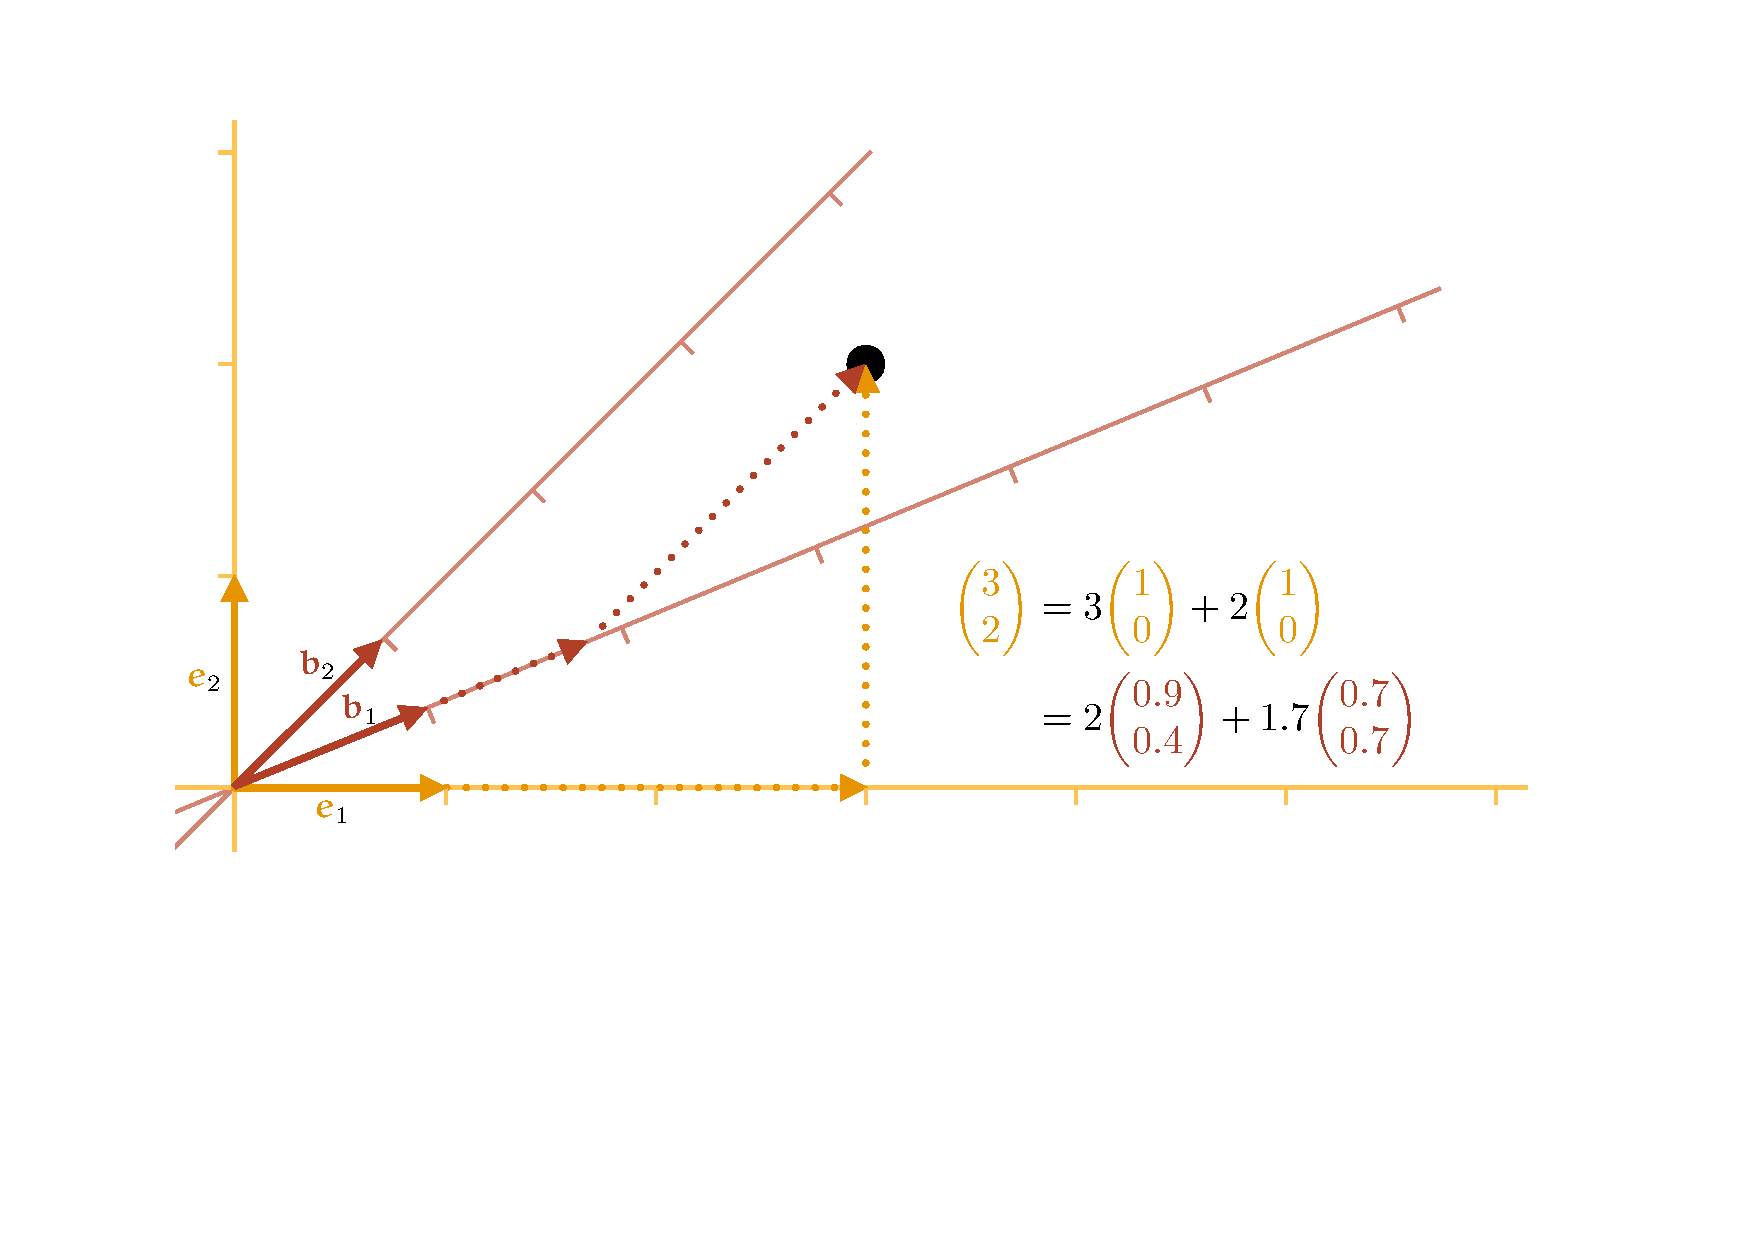
\includegraphics[width=0.7\textwidth]{./images/pca/bases.pdf}
	}
	\caption*{The point \(\oc{(3, 2)}\) as expressed in our \oc{standard basis} becomes the point \(\rc{(2, 1.7)}\) when expressed in the basis defined by vectors \(\rc{\mbb}_1 = (0.9, 0.4)\) and \(\rc{\mbb}_2 = (0.7, 0.7)\).}
\end{figure}

%<figure class="narrow">
%<img src="/images/pca/bases.svg"/>
%<figcaption>The point \(\oc{(3, 2)}\) as expressed in our <span class="oc">standard basis</span> becomes the point \(\rc{(2, 1.7)}\) when expressed in the basis defined by vectors \(\rc{\b}_1 = (0.9, 0.4)\) and \(\rc{\b}_2 = (0.7, 0.7)\).
%</figcaption>
%</figure>

If we concatenate the basis vectors into the columns of a matrix \(\rc{\mbB}\), we can express this transformation as a simple matrix multiplication:
\[
\mbp = \rc{\mbB} \mbp^\rc{B}
\]

This also suggest how to transform in the other direction: from a point in the standard basis to a point in the basis \(\rc{B}\): we require that \(\rc{\mbB}\) is invertible and use
\[
\mbp^\rc{B} = \rc{\mbB}^{-1} \mbp \p
\]

The set of points you can express in a particular basis is called its \textbf{span}. In the image above, the span is the same as that of the standard basis, but if you define two basis vectors in a three-dimensional standard basis, their span would usually be some plane crossing the origin.

\index{Span}

%<!-- 
%<aside>The strict definition of a basis states that a set \(B\) of vectors is only a basis for its span if \(B\) contains no "superfluous" vectors, i.e. vector which we can remove wihout changing the span. Another way of saying this is that no vector in \(B\) can be expressed as a linear combination of one or more of the others.
%</aside>
% -->

If you want to actually compute the transformation into the basis, the computation of a matrix inverse is finicky and very likely to be numerically unstable. It's nice if you can ensure that \(\rc{\mbB}^{-1} = \rc{\mbB}^{T}\). We've seen matrices with this property already: they're called \textbf{orthogonal matrices}. To refresh your memory, orthogonal matrices are square matrices with columns that are all unit vectors and all mutually orthogonal. 

\index{Basis!orthonormal}

\begin{aside}A basis expressed by an orthogonal matrix is called an orthonormal basis. It's a rotated or flipped version of the standard basis, but the basis vectors are still all orthogonal and they are still all unit vectors.
\end{aside}

We can now say that our data normalization was nothing more than a simple basis transformation in \({\mathbb R}^1\). We mean-center the data, and replace the standard basis vector by one that matches the variance of our data. This is not an orthonormal basis, but we'll see a fix for that later.

More importantly, we can translate the idea of data normalization to higher dimensions. 

In  \({\mathbb R}^1\), we were after a basis in which the variance was 1. In \({\mathbb R}^n\) we will look for a basis in which the \emph{covariance} is \(\mbI\). 

\pagebreak  
\noindent This requirement has two consequences: 
\begin{itemize}
\item In our new coordinates, the variance is \(1\) along all axes.
\item In our new coordinates all covariances are \(0\). That is, the data is perfectly \emph{decorrelated}.
\end{itemize}

\index{Decorrelated}

\begin{aside}This kind of normalization is called \emph{whitening} (because standard normally distributed noise is sometimes called white noise). It's not usually necessary in data science, but it can be a very powerful preprocessing method if you can spare the required resources. We're primarily discussing it as a way of making intuitive what is happening under the hood of PCA.
\end{aside}

\index{Whitening}

We'll proceed the same way we did before: we will imagine that our data was originally of this form, and has been transformed by an affine transformation. We'll call  the matrix for this imagined  ``original'' data \(\mbZ\). This means that we assume that \(\mbX\) was produced by sampling \(\mbZ\) from a standard normal distribution and transforming with as:

\[
\mbX^T = \bc{\mbA}\mbZ^T + \oc{\mbt}
\]
with some $\bc{\mbA}$ and $\oc{\mbt}$.

As before, we will first figure out which \(\bc{\mbA}\) and which \(\oc{\mbt}\) will take us from the latent data \(\mbZ\) to our observed data \(\mbX\), and then we will invert this transformation to find the transformation that normalizes our data.

The logic for \(\oc{\mbt}\) is the same as it was before: since \(\mbZ\) has zero mean, it still has zero mean after being transformed by \(\bc{\mbA}\). If we set \(\oc{\mbt} = \bar\mbx\), we transport this to the mean of the observed data.

We move this term to the left-hand side

\[
\mbX^T - \oc{\bar\mbx} = \bc{\mbA}\mbZ^T
\]

and observe that the mean-centered data on the left is equal to our \(\bc{\mbA}\)-transformed latent data.

Now, we need to set \(\bc{\mbA}\) to achieve the right covariance. The covariance is unaffected by the additive term \(- \oc{\bar \mbx}\), so we can ignore that. The covariance of the transformed data is:

\[
\text{Cov}(\mbX) = \kc{\frac{1}{n}} \bc{\mbA}\mbZ^T(\bc{\mbA}\mbZ^T)^T = \kc{\frac{1}{n}} \bc{\mbA}\mbZ^T\mbZ\bc{\mbA}^T = \bc{\mbA}\kc{\text{Cov}(\mbZ)}\bc{\mbA}^T = \bc{\mbA}\bc{\mbA}^T \p
\]

Where previously we needed to choose our scalar \(\bc{s}\) so that its square was equal to the data variance \(\bc{\sigma}^2\), we now need to choose our transformation matrix \(\bc{\mbA}\) so that its ``square'' \(\bc{\mbA}\bc{\mbA}^T\) is equal to the data \emph{co}variance \(\bc{\mbS}\).

If we find such an \(\bc{\mbA}\), we know that its \emph{transformation} is what maps the decorrelated data to the data we've observed. So even though we never transform any points by the covariance matrix, we see that internally, it does contain a very natural transformation matrix.

There are a few ways to find \(\bc{\mbA}\) for a given \(\bc{\mbS}\). The Cholesky decomposition is the most natural analogue to the square root we used in the 1D case. This road leads to a technique known as \emph{Cholesky whitening}.

\index{Whitening!Cholesky}\index{Cholesky whitening}

But this is not a book about whitening, it's a book about PCA. We're trying build some intuition for what PCA is doing. So instead, we'll solve \(\bc{\mbS} = \bc{\mbA}\bc{\mbA}^T\) using the orthogonal diagonalization we developed earlier, which will lead us to a method called \emph{PCA whitening} (a kind of byproduct of the PCA analysis).

\index{Whitening!PCA}\index{PCA!Whitening}

We know that \(\bc{\mbS}\) is square and symmetric, so we know it can be orthogonally diagonalized:

\[
\bc{\mbS} = \rc{\mbP}\bc{\mbD}\rc{\mbP}^T \p
\]

To turn this into a solution to \(\bc{\mbS} = \bc{\mbA}\bc{\mbA}^T\) we need two factors, with the second the transpose of the first. We can do this easily by noting two things about the diagonal matrix in the middle. First, the square root $\bc{\mbD}^\frac{1}{2}$ of a diagonal matrix $\bc{\mbD}$ is just another diagonal matrix with the square roots of the original elements along the diagonal. This gives us \(\bc{\mbD} = \bc{\mbD^\frac{1}{2}}\bc{\mbD^\frac{1}{2}}\). Second, the transpose of a diagonal matrix is the same matrix, so that \(\bc{\mbD} = \bc{\mbD^\frac{1}{2}}{\bc{\mbD^\frac{1}{2}}}^T\). Thus

\index{Matrix square root}\index{Square root!of a matrix}\index{$\bc{\mbA}^\frac{1}{2}$}

\begin{align*}
\bc{\mbS} &= \rc{\mbP}\bc{\mbD^\frac{1}{2}}{\bc{\mbD^\frac{1}{2}}}^T\rc{\mbP}^T \\
&= \bc{\mbA}\bc{\mbA}^T \hspace{2em}\text{with } \bc{\mbA} = \rc{\mbP}\bc{\mbD^\frac{1}{2}}
\end{align*}

Finally, to whiten our data, we reverse the transformation from \(\mbZ\) to \(\mbX\) and get 

\[
\mbZ = \bc{\mbA}^{-1}(\mbX - \oc{\mbt}) = \bc{\mbD}^{-\frac{1}{2}}\rc{\mbP}^T (\mbX - \oc{\mbt}) \p
\]

So, to map our data to a zero-mean, unit-variance, decorrelated form, we map to the basis formed by the eigenvectors of \(\bc{\mbS}\) and then divide along each axis  by the square root of the eigenvalues. We can see here that the eigenvalues of the covariance matrix are the variances of the data, \emph{along the eigenvectors} (remember that we divided by the square of the variance before).

Taking the alternative perspective we took above, we can also keep the data where it is and \emph{change our basis}. We scale the standard basis along the axes by   \(\bc{\mbD}^{\frac{1}{2}}\) rotate by \(\rc{\mbP}\) and translate by \(\oc{\bar \mbx}\). In the resulting axes, our data has mean \(\mathbf 0\), and covariance \(\mbI\).


\begin{figure}[H]
	\centerline{
	\includesvg[width=1\textwidth]{./images/pca/covariance-2.svg}
	}
\end{figure}

%<figure class="narrow">
%<img src="/images/pca/covariance-2.svg" />
%</figure>

\begin{aside}%
Note how we're having our cake and eating it too. We are scaling our axes to control the variance, so we can't have an orthonormal basis, but the eigendecomposition breaks the basis transformation in two steps: first an orthonormal basis transformation, which allows us to use $\rc{\mbP}^T$ instead of $\rc{\mbP}^{-1}$, and then a scaling along the new axes by the eigenvalues.
\end{aside}


\section{Quadratic forms}

Have we fully married our first intuition about eigenvectors in transformation matrices with the role eigenvectors play in PCA, as the eigenvectors of \(\bc{\mbS}\)? Not quite. We've shown that \(\bc{\mbS}\) is in some sense composed of a very important transformation \(\bc{\mbA}\), which transforms decorrelated data with unit variance to have covariance \(\bc{\mbS}\), but the eigenvectors we're using are not the eigenvectors of \(\bc{\mbA}\). Rather,  \(\bc{\mbA}\) is \emph{made up} of our eigenvectors and may itself have different eigenvectors, or no (real) eigenvectors at all.

\begin{aside}%
We will see in Chapter~\ref{chapter:svd} that the eigenvectors of $\bc{\mbS}$ are called the \emph{singular} vectors of $\bc{\mbA}$.
\end{aside}

\index{Singular vectors}

To develop an intuition for how \(\bc{\mbS}\) operates on space, it's more helpful not to look at the linear form

\[\bc{\mbS}\mbx\]

but at the \emph{quadratic} form 

\[\mbx^T\bc{\mbS}\mbx \p\]

\index{Quadratic form}

This may look mysterious, but it's just a concise way of writing second-order polynomials in \(n\) variables (just like \(\mbM\mbx\) is a concise way of writing a linear function from \(n\) to \(m\) variables). For instance,

\[
\mbx^T\begin{pmatrix}\rc{2}& \bc{3}\\ \gc{4}& \oc{5} \end{pmatrix}\mbx = \rc{2}{x_1}^2 + \bc{3}x_2 x_1  + \gc{4} x_1x_2 + \oc{5}{x_2}^2
\]

The simplest quadratic is \(\mbx^T\mbI\mbx\), or just \(\mbx^T\mbx\). If we set this equal to 1, the points that satisfy the resulting equation are the unit vectors. In 2 dimensions, these form a circle called the bi-unit circle. In higher dimensions, the resulting set is called the bi-unit (hyper)sphere. 

\index{Bi-unit!circle}\index{Bi-unit!sphere}

\noindent There are two ways to use quadratic forms to study the eigenvectors of \(\bc{\mbS}\). The first is to look at \(\mbx^T\bc{\mbS}\mbx\) and to study what this function looks like when constrained to the bi-unit sphere. Looking only at the points for which \(\mbx^T\mbx = 1\) what happens to the parabola \(\mbx^T\bc{\mbS}\mbx\)?

\vspace{-3.5em}
\begin{figure}[H]
	\centerline{
	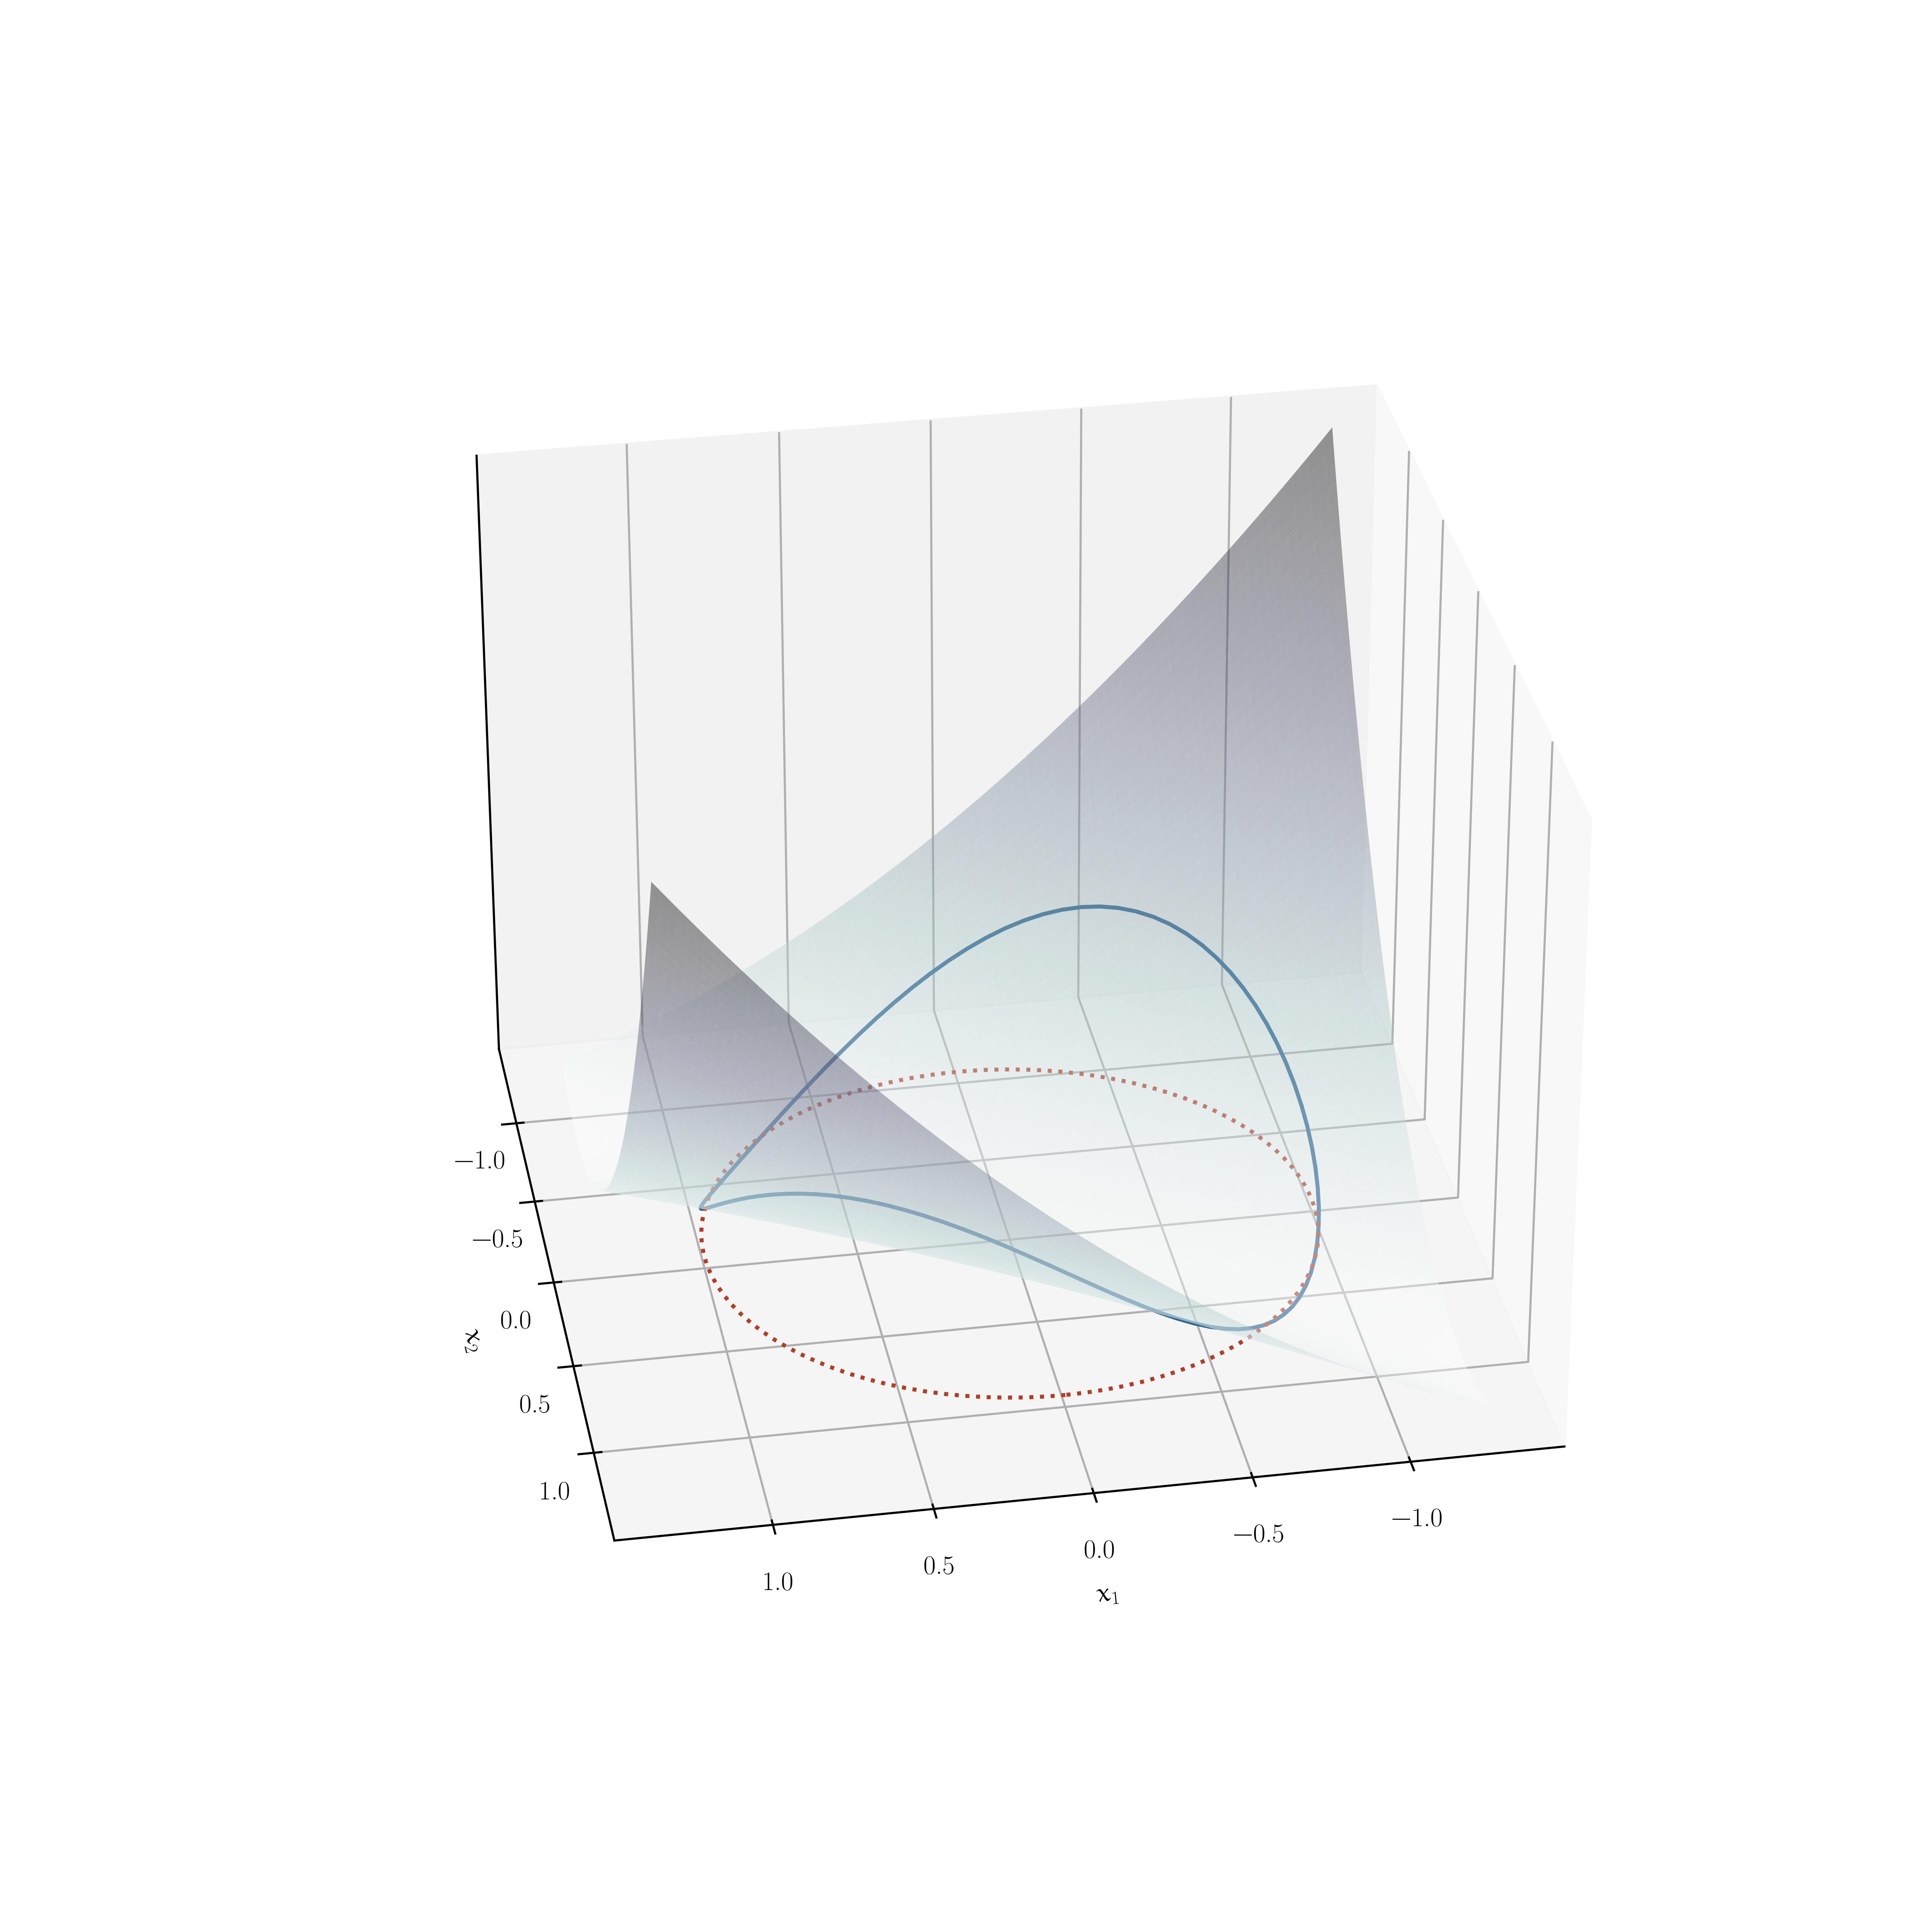
\includegraphics[width=1.2\textwidth]{./images/pca/surface.png}
	\vspace{-3.5em}
	}
	\caption*{The \bc{bi-unit circle} is deformed by the parabola \(\mbx^T\begin{pmatrix}\rc{2}& \bc{3}\\ \gc{4}& \oc{5} \end{pmatrix}\mbx\)}
\end{figure}
%<figure class="narrow">
%<img src="/images/pca/surface.svg"/>
%<figcaption>The <span class="rc">bi-unit circle</span> is deformed by the parabola \(\x^T\begin{pmatrix}\rc{2}& \bc{3}\\ \gc{4}& \oc{5} \end{pmatrix}\x\). 
%</figcaption>
%</figure>

If we diagonalize \(\bc{\mbS} = \rc{\mbP}\bc{\mbD}\rc{\mbP}^T\), the quadratic becomes \(\mbx^T\rc{\mbP}\bc{\mbD}\rc{\mbP}^T\mbx\). The first and last two factors are just a change of basis so we can also write \(\mbz^T\bc{\mbD}\mbz\) with \(\mbz = \rc{\mbP}^T\mbx\). Since \(\rc{\mbP}\) is orthogonal, the change of basis doesn't change the length of the vectors and the constraint that \(\mbx\) should be unit vectors is equivalent to requiring that \(\mbz\) be unit vectors.

\noindent The quadratic form \(\mbz\bc{\mbD}\mbz\) is particularly simple, because \(\bc{\mbD}\) is diagonal. We simply get 

\[
\mbz\bc{\mbD}\mbz = z_1z_1\bc{D}_{11} + z_2z_2\bc{D}_{22} + \ldots + z_\bc{m}z_\bc{m}\bc{D}_\bc{mm} \p
\]

\index{Quadratic form!of a diagonal matrix}

This sum is very important. Note that all the factors \(z_\bc{r}z_\bc{r}\) are not only positive (because they're squares), but they also sum to one, since \(\|
\mbz\|^2  = {z_1}^2 + \ldots + {z_\bc{m}}^2\) is the squared length of vector \(\mbz\), which we constrained to \(1\).

We'll call this a \textbf{weighted sum}: a sum over some set of numbers where each term is multiplied by a positive weight, so that the weights sum to \(1\).

\index{Weighted sum}

%<!--
% We can explain why S is acting on space as a quadratic transform and why maximizing the quadritic form maximizes the variance. Double check and add this.
% -->

In the next section, we will use this sum to prove just about every open question we have left. For now, just notice what happens when \(\mbx\) is an eigenvector. In that case, \(\mbz\) is a one-hot vector, because \(\rc{\mbP}\mbz = \mbx\), and only one of the terms in the sum is non-zero.

\index{One-hot vector}

This is one way to think of the quadratic form of \(\bc{\mbS}\): it defines \(\bc{m}\) \rc{orthogonal directions in space} (the eigenvectors), at which the quadratic takes some \bc{arbitary value} (the eigenvalues). For all other directions \(\mbx\), the quadratic is a weighted mixture  between the eigenvalues, with the weights determined by how much of \(\mbx\) projects onto the corresponding eigenvectors.

\begin{aside}Looking at the sum above, you may be able to figure out what the minimum and maximum values are of the quadratic form \(\mbx^T\bc{\mbS}\mbx\) under the constraint that \(\mbx^T\mbx = 1\). Note the similarity of this optimization problem to the PCA problem. If you don't see it yet, don't worry. We'll dig deeper into this in the next section.
\end{aside}

For another geometric interpretation of the  eigenvectors of \(\bc{\mbS}\), think back to the one-dimensional example of normalizing data. 

In the normalized version of the data, the variance is equal to \(1\). This means that, for most distributions, we can be sure that the majority of the data lies in the interval \((-1, 1)\). This is called the bi-unit interval, since it is made up of two units around the origin. If our data is normally distributed, this interval captures about 68\% of it after normalization. The transformation by \(\oc{t}\) and \(\bc{s}\) maps this interval to an interval that captures the same proportion of the unnormalized data.

\index{Bi-unit!interval}

\noindent In higher dimensions, the analogue of the bi-unit interval is the bi-unit sphere, the set of all points that are at most \(1\) away from the origin. To follow the analogy, we can transform the bi-unit sphere, which captures the majority of \(\mbZ\), by some \(\bc{\mbA}^{-1}\) so that we capture the majority of the observed data $\mbX$.

\index{Bi-unit!sphere}

\begin{figure}[H]
	\centerline{
	\includesvg[width=1\textwidth]{./images/pca/covariance-ellipses.svg}
	}
	\caption*{The \oc{bi-unit circle} captures the majority of the normalized data. The \rc{ellipse} we create by transforming the circle by \(\bc{\mbA}^{-1}\) (and translating to the mean) captures the same majority of the \gc{unnormalized data}.}
\end{figure}

%<figure class="narrow">
%<img src="/images/pca/covariance-ellipses.svg" />
%<figcaption>The <span class="oc">bi-unit circle</span> captures the majority of the normalized data. The <span class="rc">ellipse</span> we create by transforming the circle by \(\bc{\A}^{-1}\) (and translating to the mean) captures the same majority of the <span class="gc">unnormalized data</span>.
%</figcaption>
%</figure>

In two dimensions, the transformation by \(\bc{\mbA}\) and \(\oc{\mbt}\) that we derived above is the transformation that maps the bi-unit circle to an ellipse which captures the majority of the data. In more than two dimensions, we're mapping a hypersphere to an \emph{ellipsoid}.

\index{Ellipsoid}

\noindent Note that the standard basis vectors are mapped to the eigenvectors of \(\bc{\mbS}\). We call this new basis, in which the data is normalized, the \textbf{eigenbasis} of \(\bc{\mbS}\).

\index{Eigenbasis}

To work out the shape of the ellipsoid in quadratic form, we just start with the set of all unit vectors \(C = \left \{ \mbu :\mbu^T\mbu = 1 \right\}\) and transform each by \(\bc{\mbA}\) individually (much like we transformed the Mona Lisa earlier).

\vspace{-1em}
\begin{align*}
\bc{\mbA}C &= \left \{\bc{\mbA}\mbu : \mbu^T\mbI\mbu = 1 \right\} & \\
& = \left \{\mby : \mbu^T\mbu = 1 \;\;\text{and}\;\; \mby = \bc{\mbA}\mbu \right\} & \\
& = \left \{\mby :  \left ( \bc{\mbA}^{-1} \mby \right ) ^T \bc{\mbA}^{-1}\mby = 1\right \} & \\
& = \left \{\mby :  \mby^T \bc{\mbS}^{-1} \mby  = 1 \right\} &
\end{align*}

That is, to transform the bi-unit circle to an ellipsoid that covers the same proportion of \(\mbX\) as the circle did of \(\mbZ\), we turn the equation \(\mbu^T\mbu = 1\) into the equation \(\mby\bc{\mbS}^{-1}\mby = 1\). This gives us a quadratic form that desribes the ellipsoid that covers the majority of our data.

Why do we get an inversion from \(\bc{\mbS}\) to \(\bc{\mbS}^{-1}\)? Follow the transformation along the first eigenvector of \(\bc{\mbS}\). In this direction, we are multiplying the input unit vector by the square of the first eigenvalue (remember \(\bc{\mbA} = \rc{\mbP}\bc{\mbD}^\frac{1}{2}\)). To keep the vector a unit vector, we should therefore \emph{divide} by the square of the first eigenvalue. In other words, if we want to define a quadratic form for which the arguments transformed by \(\bc{\mbA}\) stay unit vectors, then the more the value of \(\mbx^T\bc{\mbS}\mbx\) grows, the more our quadratic form should shrink and vice versa.

\begin{aside}Note that the inverse of a symmetric matrix has a particularly simple expression in terms of its orthogonal diagonalization: \(\bc{\mbS}^{-1} = \left(\rc{\mbP}\bc{\mbD}\rc{\mbP}^T\right)^{-1} = \rc{\mbP}\bc{\mbD}^{-1}\rc{\mbP}^T\). That is, the eigenvectors stay the same, and we just take the reciprocals of the eigenvalues.
\end{aside}

\section{Why is PCA optimal?}

With the quadratic form added to our toolbox, we can finally start answering some of the deeper questions. Both visually, using transformations of ellipses, and formally, using the language of eigenvectors.

Let's start simply: why does the first principal component coincide with an eigenvector of \(\bc{\mbS}\)? And, while we're at it, which eigenvector does it coincide with?

Visually, this is easy to show. In the image above, we plotted the bi-unit circle, and its transformation into an ellipse that covers the same part of the observed data. The \oc{standard basis vectors} are mapped to the eigenvectors. Note that these become the axes of \rc{the ellipse}. One of the standard basis vectors is mapped to the ellipse's \emph{major axis}, the direction in which it bulges the most.The direction in which the data bulges the most is also the direction of greatest variance, and therefore the first principal component.

The proof of this fact is not very complex.

\begin{theorem}[First eigenvector.] The first principal component is the eigenvector of the covariance matrix \(\bc{\mbS}\) with the largest eigenvalue.
\end{theorem}
\begin{proof} The first principal component \(\rc{\mbw}_1\) is defined as 

\[
\argmax{\rc{\mbw}} \sum_\gc{i} \left(\rc{\mbw}^T\mbx_\gc{i}\right)^2 \\
\;\;\text{such that } \rc{\mbw}^T\rc{\mbw} = 1
\]

that is, the direction in which the variance of the projected data is maximized.

Rewriting the objective function, we get

\begin{align*}
 \sum_\gc{i} \left(\rc{\mbw}^T\mbx_\gc{i}\right)^2 &= \sum_\gc{i} \rc{\mbw}^T\mbx_\gc{i}\mbx_\gc{i}^T\rc{\mbw} \\
 &= \rc{\mbw}^T\left(\sum_\gc{i} \mbx_\gc{i}\mbx_\gc{i}^T\right)\rc{\mbw} \\
 &= \rc{\mbw}^T \mbX^T\mbX \rc{\mbw} \\
 &= \kc{N} \rc{\mbw}^T \bc{\mbS} \rc{\mbw} \p
\end{align*}

This means that the direction in which the sum of variances is maximized, is the direction, represented by a unit vector \(\rc{\mbw}\), for which the quadratic form \(\rc{\mbw}^T\bc{\mbS}\rc{\mbw}\) is maximal.

\noindent If we orthogonally diagonalize \(\bc{\mbS}\), with the eigenvalues canonically arranged, we get

\begin{align*}
\rc{\mbw}^T \bc{\mbS} \rc{\mbw} &= \rc{\mbw} ^T\rc{\mbP}\bc{\mbD}\rc{\mbP}^T \rc{\mbw} \\
&= \mbz\bc{\mbD}\mbz \;\;\text{with } \mbz = \rc{\mbP}^T\rc{\mbw} \p
\end{align*}

In the last step, we've simplified to a diagonal quadratic form in the eigenbasis of \(\bc{\mbS}\). This quadratic form simplifies to

\[
\mbz^T\bc{\mbD}\mbz = {z_1}^2 \bc{D}_{11} + \ldots + {z_\bc{m}}^2\bc{D}_\bc{mm}
\]

where the constraint that \(\mbz\) is a unit vector means that \({z_1}^2 + \ldots + {z_\bc{m}}^2 = 1\). In other words, this is a weighted sum over the diagonal elements of \(\bc{\mbD}\). To maximize a weighted sum, we assign weight \(1\) to the largest element and weight \(0\) to the rest. Since we took \(\bc{D}_{11}\) to be the largest eigenvalue, the vector \(\hat\mbz = (1, 0, \ldots, 0)\) maximizes the quadratic form.

\index{Weighted sum}

Mapping back to the standard basis, we get \(\rc{\mbw}_1 = \rc{\mbP}\hat\mbz\). That is, the first column of \(\rc{\mbP}\), which is the first eigenvector of \(\bc{\mbS}\). \hfill\qed
\end{proof}

We can extend this proof to show that all the other PCs are eigenvectors as well.

\begin{theorem}[PCs as eigenvectors.] The \(\rc{k}\)-th principal component of \(\mbX\) is the \(\rc{k}\)-th eigenvector of the covariance matrix \(\bc{\mbS}\).
\end{theorem}
\begin{proof} For the first principal component \(\rc{\mbw}_1\), the previous theorem provides a proof. For \(\rc{\mbw}_2\), follow the previous proof until the  weighted sum

\[
\mbz^T\bc{\mbD}\mbz = {z_1}^2 \bc{D}_{11} + \ldots + {z_\bc{m}}^2\bc{D}_\bc{mm} \p
\]

First, note that any vector \(\rc{\mbw}'\) that is orthogonal to \(\rc{\mbw}_1\) must also be orthogonal after transformation by \(\rc{\mbP}\rc{\mbP}^T\):
\enlargethispage{1.5em}

\[
0 = \rc{\mbw}_1^T\rc{\mbw}' = {\rc{\mbw}_1}^T\rc{\mbP}\rc{\mbP}^T\rc{\mbw}' = {\mbz_1}^T\mbz' \p
\]

Thus, the second eigenvector is orthogonal to the first (as required) if and only if their projections by \(\rc{\mbP}^T\) are orthogonal as well (and similarly for higher eigenvectors). 


Recall that the \(\mbz\)-vector of the first principal component is \((1, 0, \ldots, 0)\), so to be orthogonal, the \(\mbz\) vector corresponding to the second principal component must have \(0\) at its first element. Since the \(\bc{D}_{jj}\) are arranged in decreasing order, we maximize the sum under this constraint with the vector \(\hat \mbz = (0, 1, 0, \ldots, 0)\). \(\rc{\mbP}^T \hat\mbz\) selects the second column in \(\rc{\mbP}\), so the second principal component coincides with the second eigenvector.

The same logic holds for the other principal components. For each component \(\rc{r}\), we must set all weights \({z_i}^2\) with \(i < \rc{r}\) to zero in order for the \(\mbz\) vector to be orthogonal to all principal components already chosen. In the remainder of the sum, we maximize the weight with the one-hot vector for \(\rc{r}\), which selects the \(\rc{r}\)-th eigenvector.\hfill\qed
\end{proof}

We have finally shown that the eigenvectors are the vectors that maximize the variance. 

There is one question left to answer: Why is the set of the first \(\rc{k}\) principal components a solution to the combined problem at \(\rc{k}\)?

\begin{theorem}[Optimality of PCA.] For any \(\rc{k}\), a solution to the iterative problem is a solution to the combined problem.
\end{theorem}
\begin{proof} Let \(\rc{\mbW}\) be a solution to the combined problem at \(\rc{k}\). Let \(\mbz_1, \ldots, \mbz_\rc{k}\) be the columns of \(\rc{\mbP}^T\rc{\mbW}\), that is, the solution vectors expressed in the eigenbasis of \(\bc{\mbS}\). The total variance captured by all these \(\mbz\) is

\[\sum_\rc{r} \mbz_\rc{r}^T\bc{\mbS}\mbz_\rc{r} = \sum_{\rc{r}, \bc{j}}  {z_{\rc{r}\bc{j}} }^2\bc{D}_\bc{jj} \p
\]

Where \(z_{\rc{r}\bc{j}}\) is the \(\bc{j}\)-th element of vector \(\mbz_\rc{r}\). These are \(\rc{r}\) weighted sums, summed together. We can group the weights that each \(\mbz_\rc{r}\) contributes to each eigenvalue \(\bc{D_{jj}}\) in to a single sum:

\[
\sum_{\rc{r}, \bc{j}} {\mbz_\rc{r}}^2\bc{D}_\bc{jj} =  \sum_\bc{j} \bc{D_{jj}} \sum_\rc{r}{z_{\rc{r}\bc{j}} }^2 \p
\]

Now, since the different \(\mbz_\rc{r}\)'s are orthogonal, and each of unit length, their sum contribution to each \(\bc{D_{jj}}\) must be no more than \(1\), and the sum of each of their weights is 1.

Why? Imagine the matrix \(\mbZ\) with the \(\mbz_\rc{r}\)for its columns. What we're saying is that its squared elements of \(\mbZ\) should sum to 1 over the columns and not exceed 1 when summed over the rows. If we take \(\mbZ^T\mbZ\), the squared and summed columns end up along the diagonal. We know \(\mbZ^T\mbZ = \mbI\), so these are all \(1\).

If we take \(\mbZ\mbZ^T\), the squared and summed \emph{rows} end up along the diagonal. Extend \(\mbZ\) with orthogonal unit vectors until it is square and orthogonal. Then \(\mbZ\mbZ^T = \mbI\). Each \(1\) on the diagonal of \(\mbI\) is the result of a sum of squared values. Some come from the original \(\mbZ\), some from the columns we added, but all are squares, so it's a sum of nonnegative terms. Therefore, the terms contributed by the original vectors cannot sum to more than \(1\).


\begin{figure}[H]
	\centerline{
	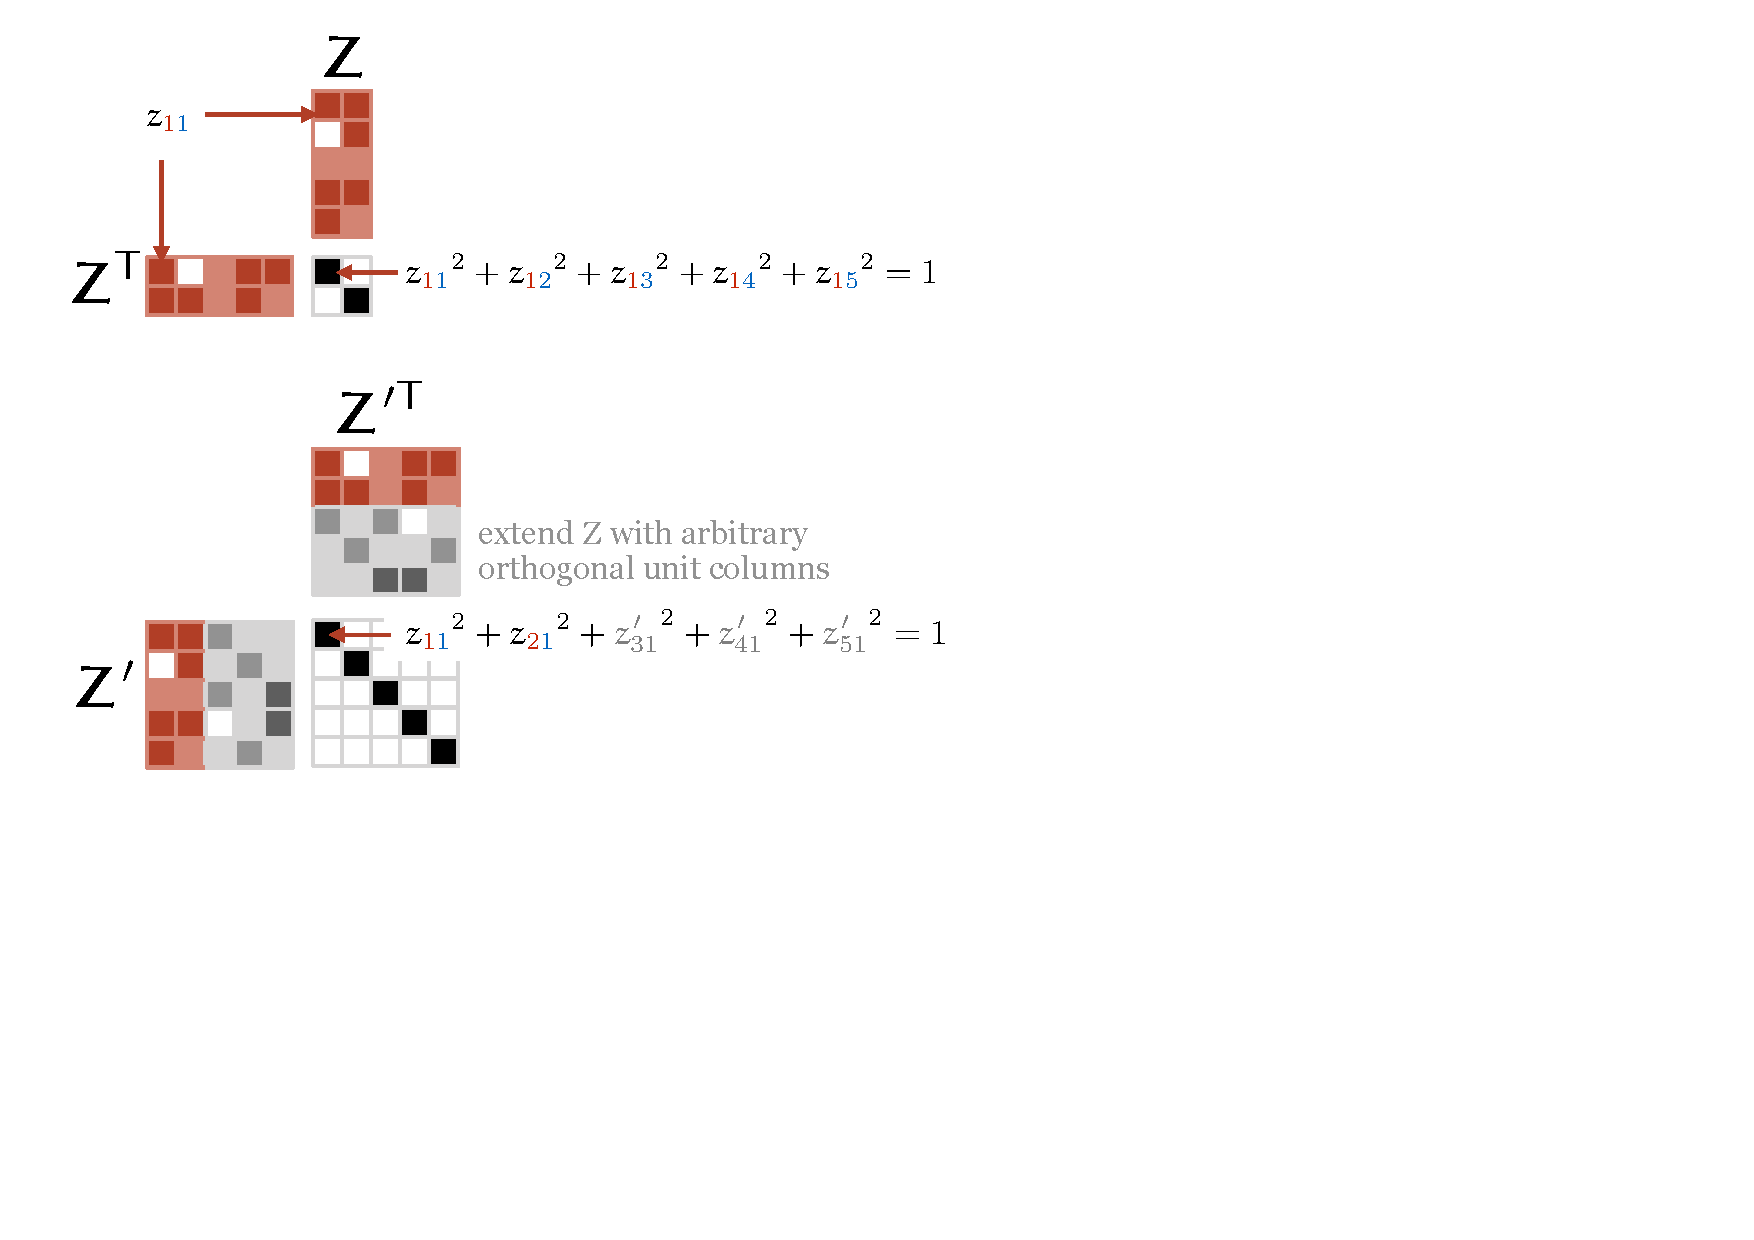
\includegraphics[width=1\textwidth]{./images/pca/zbounds.pdf}
	}
\end{figure}

%<figure class="narrow">
%<img src="/images/pca/zbounds.svg" class="three-quarters" />
%</figure>
%
So, we have a weighted sum where the total weight allowed is \(\rc{k}\), and the maximum weight per element is \(1\). The optimal solution is to give a maximum weight of \(1\) to each of the largest \(\rc{k}\) elements---that is, the first \(\rc{k}\) eigenvalues---and zero weight to everything else. 

\index{Weighted sum}

One way to achieve this is by setting \(\{\mbz_\rc{r}\}\) to be the first \(\rc{k}\) one-hot vectors, which yield the first \(\rc{k}\) eigenvectors when we transform back to the standard basis.\hfill\qed
\end{proof}

Note that when we say ``one way'' in the last paragraph, we do not mean the \emph{only} way. For instance, if we set \(\rc{k} = 2\), we get an optimum with \(\mbz_1 = (1, 0, 0, \ldots), \mbz_2 = (0, 1, 0, \ldots)\) (the PCA solution), but rotating the vectors by 45 degrees in their shared plane gives us \(\mbz_1 = (\sqrt{\small 1/2}, \sqrt{\small 1/2}, 0, \ldots), \mbz_2 = (\sqrt{\small 1/2}, -\sqrt{\small 1/2}, 0, \ldots)\). Filling these values into the sum, we see that they also result in a weight of \(1\) for \(\bc{D_{11}}\) and a weight of \(1\) for \(\bc{D_{22}}\), which means that this is also a solution to the combined problem at \(\rc{k}=2\).

More broadly, given the PCA solution, any other \(\rc{\mbW}\) whose columns span the same space as the span of the PCA solution is also a solution to the combined problem.

We have finally proved our Venn diagram correct, and we have illustrated what the rest of the light blue circle is made of.

\begin{figure}[H]
	\centerline{
	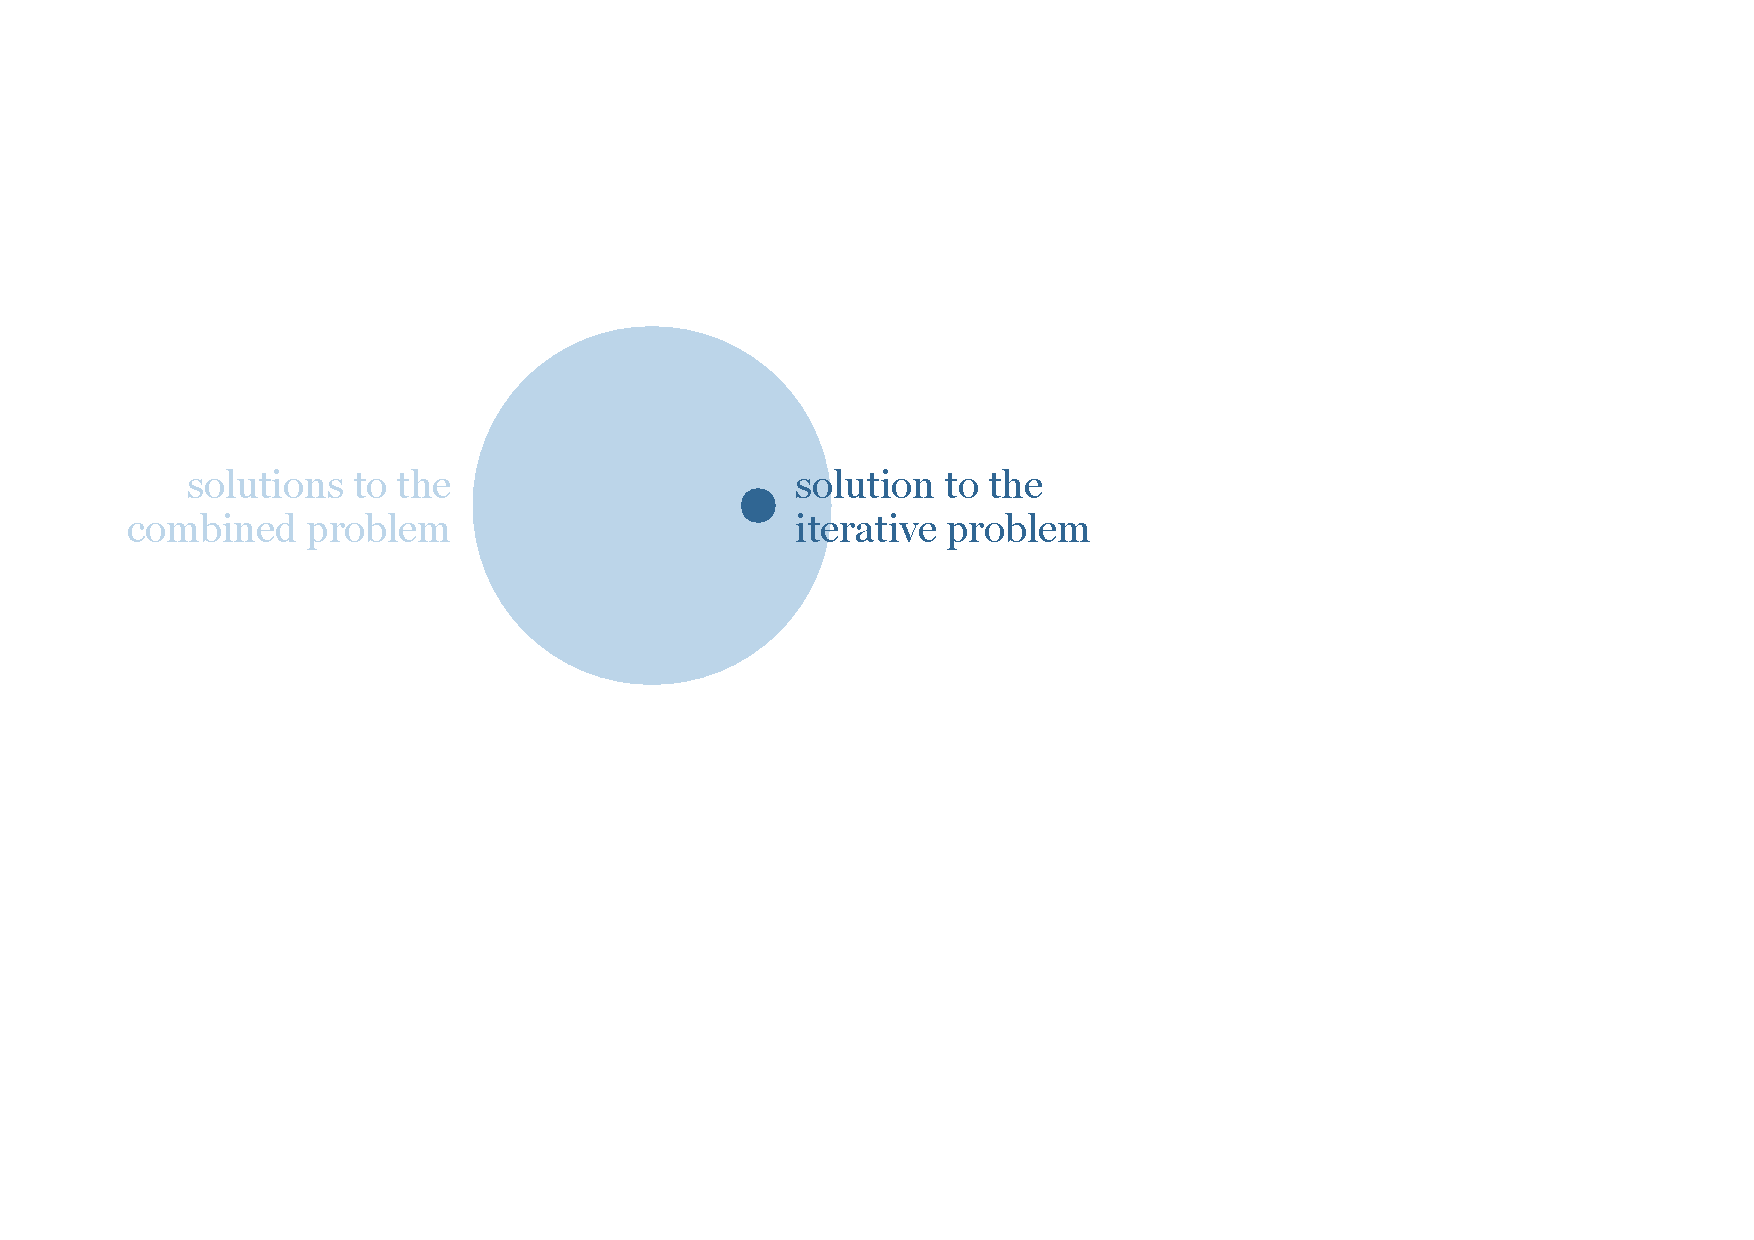
\includegraphics[width=1\textwidth]{./images/pca/venn.pdf}
	}
\end{figure}

%<figure class="narrow">
%<img src="/images/pca/venn.svg" />
%</figure>

\subsection{Characterizing the PCA solution}

Since the eigenvectors are the solution to the PCA problem, you may be forgiven for thinking of the eigenvectors  themselves in terms error minimization or variance maximization. In that case, we should guard against a misconception.

\noindent Look back at the ellipse we drew above. The first eigenvector was the major axis of the ellipse, the direction in which the data bulged out the most. However, the other eigenvector is its \emph{minor} axis. The direction in which the data bulges \emph{the least}, this makes it the direction in which the variance is \emph{minimized}.

\index{Major axis}\index{Minor axis}

To study this a bit more formally, we take the first two proofs of the previous section and turn them around. If we start with the \emph{last} eigenvector and work backward, we are choosing the directions that minimize the variance (and hence maximize the reconstruction error).

\begin{theorem}[Last eigenvector.] The direction in which the variance is minimized, is the eigenvector of \(\bc{\mbA}\) with the smallest eigenvalue.
\end{theorem}
\begin{proof}
 Follow the proof of the \textbf{\gc{first eigenvector}} theorem until the sum
 
\[
\mbz^T\bc{\mbD}\mbz = {z_1}^2 \bc{d}_{11} + \ldots + {z_\bc{m}}^2\bc{d}_\bc{mm} \p
\]

A weighted sum is minimized when all the weight is given to the smallest term. Following the same logic as before, this leads to a one-hot vector \(\hat \mbz = (0, \ldots, 0, 1)\) that selects the last column of \(\rc{\mbP}\), which is the last eigenvector.\hfill\qed
\end{proof}

Did we make a mistake somewhere? We defined the principal components as directions for which variance is maximized. Then we showed that all principal components are eigenvectors. Now we learn that at least one eigenvector actually \emph{minimizes} the variance. What gives?

\index{Variance \emph{mini}mization}

The solution lies in the fact that the sum of all variances is fixed to the sum of the variances of the data, \(z_\text{total}\). Imagine solving the combined problem for \(\rc{k} = \bc{m} - 1\). The resulting variances along the columns of the solution \(\rc{\mbW}\) should be as high as possible. However since all these columns are orthogonal, there is only one direction \(\rc{\mbv}\) left which is orthogonal to all of them. The variance along this direction, \(z_\rc{\mbv}\), is whatever variance we haven't captured in our solution:

\[
z_\rc{1} + \ldots + z_{\bc{m} - 1} + z_\rc{\mbv} = z_\text{total}
\]

Since \(z_\text{total}\) is fixed, maximizing the first \(\bc{m} - 1\) terms is equivalent to minimizing the last. 

We can define a kind of \emph{reverse iterative problem} where we define the last principal component as the direction that minimizes the variance, the last-but-one principal component as the direction orthogonal to the last principal component, the last-but-two principal component as the direction orthogonal to the last two that minimizes the variance and so on. 

\index{Reverse iteration}

We can show that optimizing for this problem gives us exactly the same vectors as optimizing for the original iterative problem which maximized the variance.

\begin{theorem}[Reverse iteration.] Under the reverse iterative problem, the last-but-\(\rc{r}\) principal component chosen coincides with the \(\rc{k}\)-th eigenvector of \(\bc{\mbS}\), with \(\rc{k} = \bc{m} - \rc{r}\), and therefore with the \(\rc{k}\)-th principal component.
\end{theorem}

The proof is the same as that of the \textbf{\gc{PCs as eigenvectors}} theorem, except starting with the smallest eigenvector instead of the largest and choosing \(\hat \mbz\) to \emph{minimize} at every step.

This shows us that it's not quite right to think of the eigenvectors as maximizing or minimizing some quantity like variance or reconstruction error (even though we've defined the principal components that way). The eigenvectors of \(\bc{\mbS}\) simply form a very natural orthonormal basis for the data, from which we can derive natural solutions to optimization objectives in both directions.

There is one question that we haven't answered yet. How do we refine the combined problem so that it coincides with the iterative problem? The one property that we use in our derivations above that is not stated in the combined problem, is that in the new basis, the data are \emph{decorrelated}. If we add this requirement to the optimization objective, we get:

\enlargethispage{3em}

\vspace{-0.5em}
\begin{align*}
\argmax{\rc{\mbW}} & \sum_\gc{i} \left( \mbx_\gc{i}^T\rc{\mbW} \right )^ 2 \\
\text{such that } & \rc{\mbW}^T\rc{\mbW} = \mbI \\
\text{and } & \kc{\frac{1}{N}}\rc{\mbW}^T\mbX^T\mbX\rc{\mbW} \text{ is diagonal.}
\end{align*}

For this problem, there is only one solution (up to negations of the principal components): the PCA solution. With this, we can finally let go of our iterative view of PCA, and embrace methods that compute all principal components in a single operation.


%\section{Conclusion}
 We have come home from a long walk. Let's settle by the fireplace and talk about all the things we've seen. 

We started with a broad idea of PCA as a method that iteratively minimizes the reconstruction error, while projecting into a lower dimensional space. For some reason, we saw last time, this works amazingly well and exposes many meaningful latent dimensions in our data. In this chapter, we showed first that minimizing reconstruction error is equivalent to maximizing variance.

We then looked at eigenvectors, and we show that the eigenvectors of the data covariance \(\bc{\mbS}\) arise naturally when we imagine that our data was originally decorrelated with unit variance in all directions. To me, this provides some intuition for why PCA works so well when it does. We can imagine that our data was constructed by sampling independent latent variables \(\mbz\) and then mixing them up linearly. In our income dataset, in the first chapter, there was one important latent variable: each person's salary. From this, we derived the monthly salary, and the majority of their quarterly income. The other latent variable captured random noise: whether people had some extra income, bonuses, etc.

\begin{figure}[H]
	\centerline{
	\includesvg[width=1\textwidth]{./images/pca/sol-w2.svg}
	}
\end{figure}

%<figure class="narrow">
%<img src="/images/pca/sol-w2.svg" />
%</figure>

We can imagine the same approach with the Olivetti faces. We get \bc{\(4096\)  features}, but under water, most of the work is done by a few \emph{latent} dimensions which are largely independent of each other: the subject's age, the direction of the light source, their apparent gender and so on. All of these can be chosen independently from each other, and are likely mostly decorrelated in the data. That is, if we don't light all women from the left, or only chose old men and young women.
\enlargethispage{13.5pt}

\index{Decorrelation}

\begin{aside}If these assumptions are violated, it may point to undesirable biases in our data. A very relevant topic at the moment. This shows that bias can be defined in terms of the assumed latent variables. Unfortunately, once the data is biased, it reduces our ability to extract the latent features, which makes it more difficult to counteract the bias.
\end{aside}

\index{Bias in data}

Since the assumptions behind our transformation from decorrelated data to the observed data are mostly correct, finding this transformation, and inverting it retrieves the latent dimensions. The greater the variance along a latent dimension, the more variance that particular ``choice'' added to the the data. The choice of the subject's age adds more variance than the lighting, and the lighting adds more variance than the gender.

The heart of the method is the spectral theorem. Without the decomposition \(\bc{\mbS} = \rc{\mbP}\bc{\mbD}\rc{\mbP}^T\), none of this would work. Proving that such a decomposition always exists for a symmetric matrix, and that every matrix for which the decomposition exists is symmetric, is not very difficult, but it takes a lot more background than we had room for here: this includes matrix determinants, the characteristic polynomial and complex numbers. In the next chapter, we will go over all these subjects carefully, building our intuition for them, and finish by thoroughly proving the spectral theorem.

Finally, you may wonder if any of these new insights help us in computing the principal component analysis. The answer is yes, the eigendecomposition \(\bc{\mbS} = \rc{\mbP}\bc{\mbD}\rc{\mbP}^T\) can be computed efficiently, and any linear algebra package allows you to do so. This gives you the principal components \(\rc{\mbP}\), and the rest is just matrix multiplication.

The eigendecomposition is certainly faster and more reliable than the projected gradient descent we've used so far, but it can still be a little numerically unstable. In practice, PCA is almost always computed by \textbf{singular value decomposition} (SVD). The SVD is such a massively useful method that it's worth looking at in more detail. It's inspired very much by everything we've set out above, but its practical applications reach far beyond just the computation of principal components. We'll develop the SVD in Chapter~\ref{chapter:svd} and provide some algorithms for computing both the eigendecomposition and the SVD in Chapter~\ref{chapter:algorithms}. 
But before all that, we'll return to the spectral theorem, and see exactly what is required to prove it.